    
    
    
    

    

    \hypertarget{matplotlib-3d}{%
\section{\texorpdfstring{\texttt{matplotlib}
3D}{matplotlib 3D}}\label{matplotlib-3d}}

    Nous poursuivons notre introduction à \texttt{matplotlib} avec les
visualisations en 3 dimensions. Comme pour la première partie sur les
fonctions en 2 dimensions, nous allons seulement paraphraser
\href{https://matplotlib.org/mpl_toolkits/mplot3d/tutorial.html}{le
tutoriel en ligne}, avec l'avantage toutefois que nous procurent les
notebooks.

    \begin{Verbatim}[commandchars=\\\{\}]
{\color{incolor}In [{\color{incolor}1}]:} \PY{c+c1}{\PYZsh{} la ration habituelle d\PYZsq{}imports}
        \PY{k+kn}{import} \PY{n+nn}{matplotlib}\PY{n+nn}{.}\PY{n+nn}{pyplot} \PY{k}{as} \PY{n+nn}{plt}
        \PY{c+c1}{\PYZsh{} et aussi numpy, même si ça n\PYZsq{}est pas strictement nécessaire}
        \PY{k+kn}{import} \PY{n+nn}{numpy} \PY{k}{as} \PY{n+nn}{np}
\end{Verbatim}


    Pour pouvoir faire des visualisations en 3D, il vous faut importer
ceci~:

    \begin{Verbatim}[commandchars=\\\{\}]
{\color{incolor}In [{\color{incolor}2}]:} \PY{c+c1}{\PYZsh{} même si l\PYZsq{}on n\PYZsq{}utilise pas explicitement}
        \PY{c+c1}{\PYZsh{} d\PYZsq{}attributs du module Axes3D}
        \PY{c+c1}{\PYZsh{} cet import est nécessaire pour faire}
        \PY{c+c1}{\PYZsh{} des visualisations en 3D}
        \PY{k+kn}{from} \PY{n+nn}{mpl\PYZus{}toolkits}\PY{n+nn}{.}\PY{n+nn}{mplot3d} \PY{k}{import} \PY{n}{Axes3D}
\end{Verbatim}


    Dans ce notebook nous allons utiliser un mode de visualisation un peu
plus élaboré, mieux intégré à l'environnement des notebooks~:

    \begin{Verbatim}[commandchars=\\\{\}]
{\color{incolor}In [{\color{incolor}3}]:} \PY{c+c1}{\PYZsh{} ce mode d\PYZsq{}interaction va nous permettre de nous déplacer}
        \PY{c+c1}{\PYZsh{} dans l\PYZsq{}espace pour voir les courbes en 3D}
        \PY{c+c1}{\PYZsh{} depuis plusieurs points de vue}
        \PY{o}{\PYZpc{}}\PY{k}{matplotlib} notebook
\end{Verbatim}


    Comme on va le voir très vite, avec ces réglages vous aurez la
possibilité d'explorer interactivement les visualisations en 3D.

    \hypertarget{un-premier-exemple-une-courbe}{%
\subsubsection{Un premier exemple~: une
courbe}\label{un-premier-exemple-une-courbe}}

    Commençons par le premier exemple du tutorial, qui nous montre comment
dessiner une ligne suivant une courbe définie de manière paramétrique
(ici, \(x\) et \(y\) sont fonctions de \(z\)). Les points importants
sont~:

\begin{itemize}
\tightlist
\item
  la composition d'un plot (plusieurs figures, chacune composée de
  plusieurs \emph{subplots}), reste bien entendu valide~; j'ai enrichi
  l'exemple initial pour mélanger un \emph{subplot} en 3D avec un
  \emph{subplot} en 2D~;
\item
  l'utilisation du paramètre
  \texttt{projection=\textquotesingle{}3d\textquotesingle{}} lorsqu'on
  crée un \emph{subplot} qui va se prêter à une visualisation en 3D~;
\item
  l'objet \emph{subplot} ainsi créé est une instance de la classe
  \texttt{Axes3DSubplot}~;
\item
  on peut envoyer à cet objet~:

  \begin{itemize}
  \tightlist
  \item
    la méthode \texttt{plot} qu'on avait déjà vue pour la dimension 2
    (c'est ce que l'on fait dans ce premier exemple)~;
  \item
    des méthodes spécifiques à la 3D, que l'on voit dans les exemples
    suivants.
  \end{itemize}
\end{itemize}

    \begin{Verbatim}[commandchars=\\\{\}]
{\color{incolor}In [{\color{incolor}4}]:} \PY{c+c1}{\PYZsh{} je choisis une taille raisonnable compte tenu de l\PYZsq{}espace}
        \PY{c+c1}{\PYZsh{} disponible dans fun\PYZhy{}mooc}
        \PY{n}{fig} \PY{o}{=} \PY{n}{plt}\PY{o}{.}\PY{n}{figure}\PY{p}{(}\PY{n}{figsize}\PY{o}{=}\PY{p}{(}\PY{l+m+mi}{6}\PY{p}{,} \PY{l+m+mi}{3}\PY{p}{)}\PY{p}{)}
        
        \PY{c+c1}{\PYZsh{} voici la façon de créer un *subplot*}
        \PY{c+c1}{\PYZsh{} qui se prête à une visualisation en 3D}
        \PY{n}{ax} \PY{o}{=} \PY{n}{fig}\PY{o}{.}\PY{n}{add\PYZus{}subplot}\PY{p}{(}\PY{l+m+mi}{121}\PY{p}{,} \PY{n}{projection}\PY{o}{=}\PY{l+s+s1}{\PYZsq{}}\PY{l+s+s1}{3d}\PY{l+s+s1}{\PYZsq{}}\PY{p}{)}
        
        \PY{c+c1}{\PYZsh{} à présent, copié de}
        \PY{c+c1}{\PYZsh{} https://matplotlib.org/mpl\PYZus{}toolkits/mplot3d/tutorial.html\PYZsh{}line\PYZhy{}plots}
        \PY{c+c1}{\PYZsh{} on crée une courbe paramétrique}
        \PY{c+c1}{\PYZsh{} où x et y sont fonctions de z}
        \PY{n}{theta} \PY{o}{=} \PY{n}{np}\PY{o}{.}\PY{n}{linspace}\PY{p}{(}\PY{o}{\PYZhy{}}\PY{l+m+mi}{4} \PY{o}{*} \PY{n}{np}\PY{o}{.}\PY{n}{pi}\PY{p}{,} \PY{l+m+mi}{4} \PY{o}{*} \PY{n}{np}\PY{o}{.}\PY{n}{pi}\PY{p}{,} \PY{l+m+mi}{100}\PY{p}{)}
        \PY{n}{z} \PY{o}{=} \PY{n}{np}\PY{o}{.}\PY{n}{linspace}\PY{p}{(}\PY{o}{\PYZhy{}}\PY{l+m+mi}{2}\PY{p}{,} \PY{l+m+mi}{2}\PY{p}{,} \PY{l+m+mi}{100}\PY{p}{)}
        \PY{n}{r} \PY{o}{=} \PY{n}{z}\PY{o}{*}\PY{o}{*}\PY{l+m+mi}{2} \PY{o}{+} \PY{l+m+mi}{1}
        \PY{n}{x} \PY{o}{=} \PY{n}{r} \PY{o}{*} \PY{n}{np}\PY{o}{.}\PY{n}{sin}\PY{p}{(}\PY{n}{theta}\PY{p}{)}
        \PY{n}{y} \PY{o}{=} \PY{n}{r} \PY{o}{*} \PY{n}{np}\PY{o}{.}\PY{n}{cos}\PY{p}{(}\PY{n}{theta}\PY{p}{)}
        \PY{c+c1}{\PYZsh{} on fait maitenant un appel à plot normal}
        \PY{c+c1}{\PYZsh{} mais avec un troisième paramètre}
        \PY{n}{ax}\PY{o}{.}\PY{n}{plot}\PY{p}{(}\PY{n}{x}\PY{p}{,} \PY{n}{y}\PY{p}{,} \PY{n}{z}\PY{p}{,} \PY{n}{label}\PY{o}{=}\PY{l+s+s1}{\PYZsq{}}\PY{l+s+s1}{parametric curve}\PY{l+s+s1}{\PYZsq{}}\PY{p}{)}
        \PY{n}{ax}\PY{o}{.}\PY{n}{legend}\PY{p}{(}\PY{p}{)}
        
        \PY{c+c1}{\PYZsh{} on peut tout à fait ajouter un plot usuel}
        \PY{c+c1}{\PYZsh{} dans un subplot, comme on l\PYZsq{}a vu pour la 2D}
        \PY{n}{ax2} \PY{o}{=} \PY{n}{fig}\PY{o}{.}\PY{n}{add\PYZus{}subplot}\PY{p}{(}\PY{l+m+mi}{122}\PY{p}{)}
        \PY{n}{x} \PY{o}{=} \PY{n}{np}\PY{o}{.}\PY{n}{linspace}\PY{p}{(}\PY{l+m+mi}{0}\PY{p}{,} \PY{l+m+mi}{10}\PY{p}{)}
        \PY{n}{y} \PY{o}{=} \PY{n}{x}\PY{o}{*}\PY{o}{*}\PY{l+m+mi}{2}
        \PY{n}{ax2}\PY{o}{.}\PY{n}{plot}\PY{p}{(}\PY{n}{x}\PY{p}{,} \PY{n}{y}\PY{p}{)}
        \PY{n}{plt}\PY{o}{.}\PY{n}{show}\PY{p}{(}\PY{p}{)}
\end{Verbatim}


    
    \begin{verbatim}
<IPython.core.display.Javascript object>
    \end{verbatim}

    
    
    \begin{verbatim}
<IPython.core.display.HTML object>
    \end{verbatim}

    
    Un autre point à remarquer est qu'avec le mode d'interaction que nous
avons choisi~:

\begin{verbatim}
%matplotlib notebook
\end{verbatim}

vous bénéficiez d'un mode d'interaction plus riche avec la figure. Par
exemple, vous pouvez cliquer dans la figure en 3D, et vous déplacer pour
changer de point de vue~; par exemple si vous sélectionnez l'outil
\texttt{Pan/Zoom} (l'outil avec 4 flèches), vous pouvez arriver à voir
ceci~:

    \begin{figure}
\centering
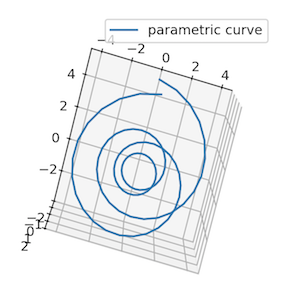
\includegraphics{media/rotated-3d.png}
\caption{rotated}
\end{figure}

    Les différents boutons d'outil
\href{https://matplotlib.org/users/navigation_toolbar.html}{sont décrits
plus en détail ici}. Je dois avouer ne pas arriver à tout utiliser
lorsque la visualisation est faite dans un notebook, mais la possibilité
de modifier le point de vue peut s'avérer intéressante pour explorer les
données.

    \begin{center}\rule{0.5\linewidth}{\linethickness}\end{center}

    En explorant les autres exemples du tutorial, vous pouvez commencer à
découvrir l'éventail des possibilités offertes par \texttt{matplotlib}.

    \hypertarget{axes3dsubplot.scatter}{%
\subsubsection{\texorpdfstring{\texttt{Axes3DSubplot.scatter}}{Axes3DSubplot.scatter}}\label{axes3dsubplot.scatter}}

    Comme en dimension 2, \texttt{scatter} permet de montrer un nuage de
points.

Tutoriel
original~:~https://matplotlib.org/mpl\_toolkits/mplot3d/tutorial.html\#scatter-plots

    \texttt{scatter3d\_demo.py}

    \begin{Verbatim}[commandchars=\\\{\}]
{\color{incolor}In [{\color{incolor}5}]:} \PY{l+s+sd}{\PYZsq{}\PYZsq{}\PYZsq{}}
        \PY{l+s+sd}{==============}
        \PY{l+s+sd}{3D scatterplot}
        \PY{l+s+sd}{==============}
        
        \PY{l+s+sd}{Demonstration of a basic scatterplot in 3D.}
        \PY{l+s+sd}{\PYZsq{}\PYZsq{}\PYZsq{}}
        
        \PY{k+kn}{from} \PY{n+nn}{mpl\PYZus{}toolkits}\PY{n+nn}{.}\PY{n+nn}{mplot3d} \PY{k}{import} \PY{n}{Axes3D}
        \PY{k+kn}{import} \PY{n+nn}{matplotlib}\PY{n+nn}{.}\PY{n+nn}{pyplot} \PY{k}{as} \PY{n+nn}{plt}
        \PY{k+kn}{import} \PY{n+nn}{numpy} \PY{k}{as} \PY{n+nn}{np}
\end{Verbatim}


    \begin{Verbatim}[commandchars=\\\{\}]
{\color{incolor}In [{\color{incolor}6}]:} \PY{n}{fig} \PY{o}{=} \PY{n}{plt}\PY{o}{.}\PY{n}{figure}\PY{p}{(}\PY{n}{figsize}\PY{o}{=}\PY{p}{(}\PY{l+m+mi}{4}\PY{p}{,} \PY{l+m+mi}{4}\PY{p}{)}\PY{p}{)}
        
        \PY{k}{def} \PY{n+nf}{randrange}\PY{p}{(}\PY{n}{n}\PY{p}{,} \PY{n}{vmin}\PY{p}{,} \PY{n}{vmax}\PY{p}{)}\PY{p}{:}
            \PY{l+s+sd}{\PYZsq{}\PYZsq{}\PYZsq{}}
        \PY{l+s+sd}{    Helper function to make an array of random numbers having shape (n, )}
        \PY{l+s+sd}{    with each number distributed Uniform(vmin, vmax).}
        \PY{l+s+sd}{    \PYZsq{}\PYZsq{}\PYZsq{}}
            \PY{k}{return} \PY{p}{(}\PY{n}{vmax} \PY{o}{\PYZhy{}} \PY{n}{vmin}\PY{p}{)}\PY{o}{*}\PY{n}{np}\PY{o}{.}\PY{n}{random}\PY{o}{.}\PY{n}{rand}\PY{p}{(}\PY{n}{n}\PY{p}{)} \PY{o}{+} \PY{n}{vmin}
        
        \PY{n}{ax} \PY{o}{=} \PY{n}{fig}\PY{o}{.}\PY{n}{add\PYZus{}subplot}\PY{p}{(}\PY{l+m+mi}{111}\PY{p}{,} \PY{n}{projection}\PY{o}{=}\PY{l+s+s1}{\PYZsq{}}\PY{l+s+s1}{3d}\PY{l+s+s1}{\PYZsq{}}\PY{p}{)}
        
        \PY{n}{n} \PY{o}{=} \PY{l+m+mi}{100}
        
        \PY{c+c1}{\PYZsh{} For each set of style and range settings, plot n random points in the box}
        \PY{c+c1}{\PYZsh{} defined by x in [23, 32], y in [0, 100], z in [zlow, zhigh].}
        \PY{k}{for} \PY{n}{c}\PY{p}{,} \PY{n}{m}\PY{p}{,} \PY{n}{zlow}\PY{p}{,} \PY{n}{zhigh} \PY{o+ow}{in} \PY{p}{[}\PY{p}{(}\PY{l+s+s1}{\PYZsq{}}\PY{l+s+s1}{r}\PY{l+s+s1}{\PYZsq{}}\PY{p}{,} \PY{l+s+s1}{\PYZsq{}}\PY{l+s+s1}{o}\PY{l+s+s1}{\PYZsq{}}\PY{p}{,} \PY{o}{\PYZhy{}}\PY{l+m+mi}{50}\PY{p}{,} \PY{o}{\PYZhy{}}\PY{l+m+mi}{25}\PY{p}{)}\PY{p}{,} \PY{p}{(}\PY{l+s+s1}{\PYZsq{}}\PY{l+s+s1}{b}\PY{l+s+s1}{\PYZsq{}}\PY{p}{,} \PY{l+s+s1}{\PYZsq{}}\PY{l+s+s1}{\PYZca{}}\PY{l+s+s1}{\PYZsq{}}\PY{p}{,} \PY{o}{\PYZhy{}}\PY{l+m+mi}{30}\PY{p}{,} \PY{o}{\PYZhy{}}\PY{l+m+mi}{5}\PY{p}{)}\PY{p}{]}\PY{p}{:}
            \PY{n}{xs} \PY{o}{=} \PY{n}{randrange}\PY{p}{(}\PY{n}{n}\PY{p}{,} \PY{l+m+mi}{23}\PY{p}{,} \PY{l+m+mi}{32}\PY{p}{)}
            \PY{n}{ys} \PY{o}{=} \PY{n}{randrange}\PY{p}{(}\PY{n}{n}\PY{p}{,} \PY{l+m+mi}{0}\PY{p}{,} \PY{l+m+mi}{100}\PY{p}{)}
            \PY{n}{zs} \PY{o}{=} \PY{n}{randrange}\PY{p}{(}\PY{n}{n}\PY{p}{,} \PY{n}{zlow}\PY{p}{,} \PY{n}{zhigh}\PY{p}{)}
            \PY{n}{ax}\PY{o}{.}\PY{n}{scatter}\PY{p}{(}\PY{n}{xs}\PY{p}{,} \PY{n}{ys}\PY{p}{,} \PY{n}{zs}\PY{p}{,} \PY{n}{c}\PY{o}{=}\PY{n}{c}\PY{p}{,} \PY{n}{marker}\PY{o}{=}\PY{n}{m}\PY{p}{)}
        
        \PY{n}{ax}\PY{o}{.}\PY{n}{set\PYZus{}xlabel}\PY{p}{(}\PY{l+s+s1}{\PYZsq{}}\PY{l+s+s1}{X Label}\PY{l+s+s1}{\PYZsq{}}\PY{p}{)}
        \PY{n}{plt}\PY{o}{.}\PY{n}{show}\PY{p}{(}\PY{p}{)}
\end{Verbatim}


    
    \begin{verbatim}
<IPython.core.display.Javascript object>
    \end{verbatim}

    
    
    \begin{verbatim}
<IPython.core.display.HTML object>
    \end{verbatim}

    
    \hypertarget{axes3dsubplot.plot_wireframe}{%
\subsubsection{\texorpdfstring{\texttt{Axes3DSubplot.plot\_wireframe}}{Axes3DSubplot.plot\_wireframe}}\label{axes3dsubplot.plot_wireframe}}

    Utilisez cette méthode pour dessiner en mode ``fil de fer''.

    Tutoriel
original~:~\url{https://matplotlib.org/mpl_toolkits/mplot3d/tutorial.html\#wireframe-plots}.

    \texttt{wire3d\_demo.py}

    \begin{Verbatim}[commandchars=\\\{\}]
{\color{incolor}In [{\color{incolor}7}]:} \PY{k+kn}{from} \PY{n+nn}{mpl\PYZus{}toolkits}\PY{n+nn}{.}\PY{n+nn}{mplot3d} \PY{k}{import} \PY{n}{axes3d}
\end{Verbatim}


    \begin{Verbatim}[commandchars=\\\{\}]
{\color{incolor}In [{\color{incolor}8}]:} \PY{n}{fig} \PY{o}{=} \PY{n}{plt}\PY{o}{.}\PY{n}{figure}\PY{p}{(}\PY{n}{figsize}\PY{o}{=}\PY{p}{(}\PY{l+m+mi}{4}\PY{p}{,} \PY{l+m+mi}{4}\PY{p}{)}\PY{p}{)}
        
        \PY{n}{ax} \PY{o}{=} \PY{n}{fig}\PY{o}{.}\PY{n}{add\PYZus{}subplot}\PY{p}{(}\PY{l+m+mi}{111}\PY{p}{,} \PY{n}{projection}\PY{o}{=}\PY{l+s+s1}{\PYZsq{}}\PY{l+s+s1}{3d}\PY{l+s+s1}{\PYZsq{}}\PY{p}{)}
        
        \PY{c+c1}{\PYZsh{} Grab some test data.}
        \PY{n}{X}\PY{p}{,} \PY{n}{Y}\PY{p}{,} \PY{n}{Z} \PY{o}{=} \PY{n}{axes3d}\PY{o}{.}\PY{n}{get\PYZus{}test\PYZus{}data}\PY{p}{(}\PY{l+m+mf}{0.05}\PY{p}{)}
        
        \PY{c+c1}{\PYZsh{} Plot a basic wireframe.}
        \PY{n}{ax}\PY{o}{.}\PY{n}{plot\PYZus{}wireframe}\PY{p}{(}\PY{n}{X}\PY{p}{,} \PY{n}{Y}\PY{p}{,} \PY{n}{Z}\PY{p}{,} \PY{n}{rstride}\PY{o}{=}\PY{l+m+mi}{10}\PY{p}{,} \PY{n}{cstride}\PY{o}{=}\PY{l+m+mi}{10}\PY{p}{)}
        \PY{n}{plt}\PY{o}{.}\PY{n}{show}\PY{p}{(}\PY{p}{)}
\end{Verbatim}


    
    \begin{verbatim}
<IPython.core.display.Javascript object>
    \end{verbatim}

    
    
    \begin{verbatim}
<IPython.core.display.HTML object>
    \end{verbatim}

    
    \hypertarget{axes3dsubplot.plot_surface}{%
\subsubsection{\texorpdfstring{\texttt{Axes3DSubplot.plot\_surface}}{Axes3DSubplot.plot\_surface}}\label{axes3dsubplot.plot_surface}}

    Comme on s'en doute, \texttt{plot\_surface} sert à dessiner des surfaces
dans l'espace~; ces exemples montrent surtout comment utiliser des
couleurs ou des \emph{patterns}.

    Tutoriel
original~:~\url{https://matplotlib.org/mpl_toolkits/mplot3d/tutorial.html\#surface-plots}.

    \texttt{surface3d\_demo.py}

    \begin{Verbatim}[commandchars=\\\{\}]
{\color{incolor}In [{\color{incolor}9}]:} \PY{l+s+sd}{\PYZsq{}\PYZsq{}\PYZsq{}}
        \PY{l+s+sd}{======================}
        \PY{l+s+sd}{3D surface (color map)}
        \PY{l+s+sd}{======================}
        
        \PY{l+s+sd}{Demonstrates plotting a 3D surface colored with the coolwarm color map.}
        \PY{l+s+sd}{The surface is made opaque by using antialiased=False.}
        
        \PY{l+s+sd}{Also demonstrates using the LinearLocator and custom formatting for the}
        \PY{l+s+sd}{z axis tick labels.}
        \PY{l+s+sd}{\PYZsq{}\PYZsq{}\PYZsq{}}
        
        \PY{k+kn}{from} \PY{n+nn}{mpl\PYZus{}toolkits}\PY{n+nn}{.}\PY{n+nn}{mplot3d} \PY{k}{import} \PY{n}{Axes3D}
        \PY{k+kn}{import} \PY{n+nn}{matplotlib}\PY{n+nn}{.}\PY{n+nn}{pyplot} \PY{k}{as} \PY{n+nn}{plt}
        \PY{k+kn}{from} \PY{n+nn}{matplotlib} \PY{k}{import} \PY{n}{cm}
        \PY{k+kn}{from} \PY{n+nn}{matplotlib}\PY{n+nn}{.}\PY{n+nn}{ticker} \PY{k}{import} \PY{n}{LinearLocator}\PY{p}{,} \PY{n}{FormatStrFormatter}
        \PY{k+kn}{import} \PY{n+nn}{numpy} \PY{k}{as} \PY{n+nn}{np}
\end{Verbatim}


    \begin{Verbatim}[commandchars=\\\{\}]
{\color{incolor}In [{\color{incolor}10}]:} \PY{n}{fig} \PY{o}{=} \PY{n}{plt}\PY{o}{.}\PY{n}{figure}\PY{p}{(}\PY{n}{figsize}\PY{o}{=}\PY{p}{(}\PY{l+m+mi}{4}\PY{p}{,} \PY{l+m+mi}{4}\PY{p}{)}\PY{p}{)}
         
         \PY{n}{ax} \PY{o}{=} \PY{n}{fig}\PY{o}{.}\PY{n}{gca}\PY{p}{(}\PY{n}{projection}\PY{o}{=}\PY{l+s+s1}{\PYZsq{}}\PY{l+s+s1}{3d}\PY{l+s+s1}{\PYZsq{}}\PY{p}{)}
         
         \PY{c+c1}{\PYZsh{} Make data.}
         \PY{n}{X} \PY{o}{=} \PY{n}{np}\PY{o}{.}\PY{n}{arange}\PY{p}{(}\PY{o}{\PYZhy{}}\PY{l+m+mi}{5}\PY{p}{,} \PY{l+m+mi}{5}\PY{p}{,} \PY{l+m+mf}{0.25}\PY{p}{)}
         \PY{n}{Y} \PY{o}{=} \PY{n}{np}\PY{o}{.}\PY{n}{arange}\PY{p}{(}\PY{o}{\PYZhy{}}\PY{l+m+mi}{5}\PY{p}{,} \PY{l+m+mi}{5}\PY{p}{,} \PY{l+m+mf}{0.25}\PY{p}{)}
         \PY{n}{X}\PY{p}{,} \PY{n}{Y} \PY{o}{=} \PY{n}{np}\PY{o}{.}\PY{n}{meshgrid}\PY{p}{(}\PY{n}{X}\PY{p}{,} \PY{n}{Y}\PY{p}{)}
         \PY{n}{R} \PY{o}{=} \PY{n}{np}\PY{o}{.}\PY{n}{sqrt}\PY{p}{(}\PY{n}{X}\PY{o}{*}\PY{o}{*}\PY{l+m+mi}{2} \PY{o}{+} \PY{n}{Y}\PY{o}{*}\PY{o}{*}\PY{l+m+mi}{2}\PY{p}{)}
         \PY{n}{Z} \PY{o}{=} \PY{n}{np}\PY{o}{.}\PY{n}{sin}\PY{p}{(}\PY{n}{R}\PY{p}{)}
         
         \PY{c+c1}{\PYZsh{} Plot the surface.}
         \PY{n}{surf} \PY{o}{=} \PY{n}{ax}\PY{o}{.}\PY{n}{plot\PYZus{}surface}\PY{p}{(}\PY{n}{X}\PY{p}{,} \PY{n}{Y}\PY{p}{,} \PY{n}{Z}\PY{p}{,} \PY{n}{cmap}\PY{o}{=}\PY{n}{cm}\PY{o}{.}\PY{n}{coolwarm}\PY{p}{,}
                                \PY{n}{linewidth}\PY{o}{=}\PY{l+m+mi}{0}\PY{p}{,} \PY{n}{antialiased}\PY{o}{=}\PY{k+kc}{False}\PY{p}{)}
         
         \PY{c+c1}{\PYZsh{} Customize the z axis.}
         \PY{n}{ax}\PY{o}{.}\PY{n}{set\PYZus{}zlim}\PY{p}{(}\PY{o}{\PYZhy{}}\PY{l+m+mf}{1.01}\PY{p}{,} \PY{l+m+mf}{1.01}\PY{p}{)}
         \PY{n}{ax}\PY{o}{.}\PY{n}{zaxis}\PY{o}{.}\PY{n}{set\PYZus{}major\PYZus{}locator}\PY{p}{(}\PY{n}{LinearLocator}\PY{p}{(}\PY{l+m+mi}{10}\PY{p}{)}\PY{p}{)}
         \PY{n}{ax}\PY{o}{.}\PY{n}{zaxis}\PY{o}{.}\PY{n}{set\PYZus{}major\PYZus{}formatter}\PY{p}{(}\PY{n}{FormatStrFormatter}\PY{p}{(}\PY{l+s+s1}{\PYZsq{}}\PY{l+s+si}{\PYZpc{}.02f}\PY{l+s+s1}{\PYZsq{}}\PY{p}{)}\PY{p}{)}
         
         \PY{c+c1}{\PYZsh{} Add a color bar which maps values to colors.}
         \PY{n}{fig}\PY{o}{.}\PY{n}{colorbar}\PY{p}{(}\PY{n}{surf}\PY{p}{,} \PY{n}{shrink}\PY{o}{=}\PY{l+m+mf}{0.5}\PY{p}{,} \PY{n}{aspect}\PY{o}{=}\PY{l+m+mi}{5}\PY{p}{)}
         
         \PY{n}{plt}\PY{o}{.}\PY{n}{show}\PY{p}{(}\PY{p}{)}
\end{Verbatim}


    
    \begin{verbatim}
<IPython.core.display.Javascript object>
    \end{verbatim}

    
    
    \begin{verbatim}
<IPython.core.display.HTML object>
    \end{verbatim}

    
    \texttt{surface3d\_demo2.py}

    \begin{Verbatim}[commandchars=\\\{\}]
{\color{incolor}In [{\color{incolor}11}]:} \PY{l+s+sd}{\PYZsq{}\PYZsq{}\PYZsq{}}
         \PY{l+s+sd}{========================}
         \PY{l+s+sd}{3D surface (solid color)}
         \PY{l+s+sd}{========================}
         
         \PY{l+s+sd}{Demonstrates a very basic plot of a 3D surface using a solid color.}
         \PY{l+s+sd}{\PYZsq{}\PYZsq{}\PYZsq{}}
         
         \PY{k+kn}{from} \PY{n+nn}{mpl\PYZus{}toolkits}\PY{n+nn}{.}\PY{n+nn}{mplot3d} \PY{k}{import} \PY{n}{Axes3D}
         \PY{k+kn}{import} \PY{n+nn}{matplotlib}\PY{n+nn}{.}\PY{n+nn}{pyplot} \PY{k}{as} \PY{n+nn}{plt}
         \PY{k+kn}{import} \PY{n+nn}{numpy} \PY{k}{as} \PY{n+nn}{np}
\end{Verbatim}


    \begin{Verbatim}[commandchars=\\\{\}]
{\color{incolor}In [{\color{incolor}12}]:} \PY{n}{fig} \PY{o}{=} \PY{n}{plt}\PY{o}{.}\PY{n}{figure}\PY{p}{(}\PY{n}{figsize}\PY{o}{=}\PY{p}{(}\PY{l+m+mi}{4}\PY{p}{,} \PY{l+m+mi}{4}\PY{p}{)}\PY{p}{)}
         \PY{n}{ax} \PY{o}{=} \PY{n}{fig}\PY{o}{.}\PY{n}{add\PYZus{}subplot}\PY{p}{(}\PY{l+m+mi}{111}\PY{p}{,} \PY{n}{projection}\PY{o}{=}\PY{l+s+s1}{\PYZsq{}}\PY{l+s+s1}{3d}\PY{l+s+s1}{\PYZsq{}}\PY{p}{)}
         
         \PY{c+c1}{\PYZsh{} Make data}
         \PY{n}{u} \PY{o}{=} \PY{n}{np}\PY{o}{.}\PY{n}{linspace}\PY{p}{(}\PY{l+m+mi}{0}\PY{p}{,} \PY{l+m+mi}{2} \PY{o}{*} \PY{n}{np}\PY{o}{.}\PY{n}{pi}\PY{p}{,} \PY{l+m+mi}{30}\PY{p}{)}
         \PY{n}{v} \PY{o}{=} \PY{n}{np}\PY{o}{.}\PY{n}{linspace}\PY{p}{(}\PY{l+m+mi}{0}\PY{p}{,} \PY{n}{np}\PY{o}{.}\PY{n}{pi}\PY{p}{,} \PY{l+m+mi}{30}\PY{p}{)}
         \PY{n}{x} \PY{o}{=} \PY{l+m+mi}{10} \PY{o}{*} \PY{n}{np}\PY{o}{.}\PY{n}{outer}\PY{p}{(}\PY{n}{np}\PY{o}{.}\PY{n}{cos}\PY{p}{(}\PY{n}{u}\PY{p}{)}\PY{p}{,} \PY{n}{np}\PY{o}{.}\PY{n}{sin}\PY{p}{(}\PY{n}{v}\PY{p}{)}\PY{p}{)}
         \PY{n}{y} \PY{o}{=} \PY{l+m+mi}{10} \PY{o}{*} \PY{n}{np}\PY{o}{.}\PY{n}{outer}\PY{p}{(}\PY{n}{np}\PY{o}{.}\PY{n}{sin}\PY{p}{(}\PY{n}{u}\PY{p}{)}\PY{p}{,} \PY{n}{np}\PY{o}{.}\PY{n}{sin}\PY{p}{(}\PY{n}{v}\PY{p}{)}\PY{p}{)}
         \PY{n}{z} \PY{o}{=} \PY{l+m+mi}{10} \PY{o}{*} \PY{n}{np}\PY{o}{.}\PY{n}{outer}\PY{p}{(}\PY{n}{np}\PY{o}{.}\PY{n}{ones}\PY{p}{(}\PY{n}{np}\PY{o}{.}\PY{n}{size}\PY{p}{(}\PY{n}{u}\PY{p}{)}\PY{p}{)}\PY{p}{,} \PY{n}{np}\PY{o}{.}\PY{n}{cos}\PY{p}{(}\PY{n}{v}\PY{p}{)}\PY{p}{)}
         
         \PY{c+c1}{\PYZsh{} Plot the surface}
         \PY{n}{ax}\PY{o}{.}\PY{n}{plot\PYZus{}surface}\PY{p}{(}\PY{n}{x}\PY{p}{,} \PY{n}{y}\PY{p}{,} \PY{n}{z}\PY{p}{,} \PY{n}{color}\PY{o}{=}\PY{l+s+s1}{\PYZsq{}}\PY{l+s+s1}{b}\PY{l+s+s1}{\PYZsq{}}\PY{p}{)}
         
         \PY{n}{plt}\PY{o}{.}\PY{n}{show}\PY{p}{(}\PY{p}{)}
\end{Verbatim}


    
    \begin{verbatim}
<IPython.core.display.Javascript object>
    \end{verbatim}

    
    
    \begin{verbatim}
<IPython.core.display.HTML object>
    \end{verbatim}

    
    \texttt{surface3d\_demo3.py}

    \begin{Verbatim}[commandchars=\\\{\}]
{\color{incolor}In [{\color{incolor}13}]:} \PY{l+s+sd}{\PYZsq{}\PYZsq{}\PYZsq{}}
         \PY{l+s+sd}{=========================}
         \PY{l+s+sd}{3D surface (checkerboard)}
         \PY{l+s+sd}{=========================}
         
         \PY{l+s+sd}{Demonstrates plotting a 3D surface colored in a checkerboard pattern.}
         \PY{l+s+sd}{\PYZsq{}\PYZsq{}\PYZsq{}}
         
         \PY{k+kn}{from} \PY{n+nn}{mpl\PYZus{}toolkits}\PY{n+nn}{.}\PY{n+nn}{mplot3d} \PY{k}{import} \PY{n}{Axes3D}
         \PY{k+kn}{import} \PY{n+nn}{matplotlib}\PY{n+nn}{.}\PY{n+nn}{pyplot} \PY{k}{as} \PY{n+nn}{plt}
         \PY{k+kn}{from} \PY{n+nn}{matplotlib} \PY{k}{import} \PY{n}{cm}
         \PY{k+kn}{from} \PY{n+nn}{matplotlib}\PY{n+nn}{.}\PY{n+nn}{ticker} \PY{k}{import} \PY{n}{LinearLocator}
         \PY{k+kn}{import} \PY{n+nn}{numpy} \PY{k}{as} \PY{n+nn}{np}
\end{Verbatim}


    \begin{Verbatim}[commandchars=\\\{\}]
{\color{incolor}In [{\color{incolor}14}]:} \PY{n}{fig} \PY{o}{=} \PY{n}{plt}\PY{o}{.}\PY{n}{figure}\PY{p}{(}\PY{n}{figsize}\PY{o}{=}\PY{p}{(}\PY{l+m+mi}{4}\PY{p}{,} \PY{l+m+mi}{4}\PY{p}{)}\PY{p}{)}
         \PY{n}{ax} \PY{o}{=} \PY{n}{fig}\PY{o}{.}\PY{n}{gca}\PY{p}{(}\PY{n}{projection}\PY{o}{=}\PY{l+s+s1}{\PYZsq{}}\PY{l+s+s1}{3d}\PY{l+s+s1}{\PYZsq{}}\PY{p}{)}
         
         \PY{c+c1}{\PYZsh{} Make data.}
         \PY{n}{X} \PY{o}{=} \PY{n}{np}\PY{o}{.}\PY{n}{arange}\PY{p}{(}\PY{o}{\PYZhy{}}\PY{l+m+mi}{5}\PY{p}{,} \PY{l+m+mi}{5}\PY{p}{,} \PY{l+m+mf}{0.25}\PY{p}{)}
         \PY{n}{xlen} \PY{o}{=} \PY{n+nb}{len}\PY{p}{(}\PY{n}{X}\PY{p}{)}
         \PY{n}{Y} \PY{o}{=} \PY{n}{np}\PY{o}{.}\PY{n}{arange}\PY{p}{(}\PY{o}{\PYZhy{}}\PY{l+m+mi}{5}\PY{p}{,} \PY{l+m+mi}{5}\PY{p}{,} \PY{l+m+mf}{0.25}\PY{p}{)}
         \PY{n}{ylen} \PY{o}{=} \PY{n+nb}{len}\PY{p}{(}\PY{n}{Y}\PY{p}{)}
         \PY{n}{X}\PY{p}{,} \PY{n}{Y} \PY{o}{=} \PY{n}{np}\PY{o}{.}\PY{n}{meshgrid}\PY{p}{(}\PY{n}{X}\PY{p}{,} \PY{n}{Y}\PY{p}{)}
         \PY{n}{R} \PY{o}{=} \PY{n}{np}\PY{o}{.}\PY{n}{sqrt}\PY{p}{(}\PY{n}{X}\PY{o}{*}\PY{o}{*}\PY{l+m+mi}{2} \PY{o}{+} \PY{n}{Y}\PY{o}{*}\PY{o}{*}\PY{l+m+mi}{2}\PY{p}{)}
         \PY{n}{Z} \PY{o}{=} \PY{n}{np}\PY{o}{.}\PY{n}{sin}\PY{p}{(}\PY{n}{R}\PY{p}{)}
         
         \PY{c+c1}{\PYZsh{} Create an empty array of strings with the same shape as the meshgrid, and}
         \PY{c+c1}{\PYZsh{} populate it with two colors in a checkerboard pattern.}
         \PY{n}{colortuple} \PY{o}{=} \PY{p}{(}\PY{l+s+s1}{\PYZsq{}}\PY{l+s+s1}{y}\PY{l+s+s1}{\PYZsq{}}\PY{p}{,} \PY{l+s+s1}{\PYZsq{}}\PY{l+s+s1}{b}\PY{l+s+s1}{\PYZsq{}}\PY{p}{)}
         \PY{n}{colors} \PY{o}{=} \PY{n}{np}\PY{o}{.}\PY{n}{empty}\PY{p}{(}\PY{n}{X}\PY{o}{.}\PY{n}{shape}\PY{p}{,} \PY{n}{dtype}\PY{o}{=}\PY{n+nb}{str}\PY{p}{)}
         \PY{k}{for} \PY{n}{y} \PY{o+ow}{in} \PY{n+nb}{range}\PY{p}{(}\PY{n}{ylen}\PY{p}{)}\PY{p}{:}
             \PY{k}{for} \PY{n}{x} \PY{o+ow}{in} \PY{n+nb}{range}\PY{p}{(}\PY{n}{xlen}\PY{p}{)}\PY{p}{:}
                 \PY{n}{colors}\PY{p}{[}\PY{n}{x}\PY{p}{,} \PY{n}{y}\PY{p}{]} \PY{o}{=} \PY{n}{colortuple}\PY{p}{[}\PY{p}{(}\PY{n}{x} \PY{o}{+} \PY{n}{y}\PY{p}{)} \PY{o}{\PYZpc{}} \PY{n+nb}{len}\PY{p}{(}\PY{n}{colortuple}\PY{p}{)}\PY{p}{]}
         
         \PY{c+c1}{\PYZsh{} Plot the surface with face colors taken from the array we made.}
         \PY{n}{surf} \PY{o}{=} \PY{n}{ax}\PY{o}{.}\PY{n}{plot\PYZus{}surface}\PY{p}{(}\PY{n}{X}\PY{p}{,} \PY{n}{Y}\PY{p}{,} \PY{n}{Z}\PY{p}{,} \PY{n}{facecolors}\PY{o}{=}\PY{n}{colors}\PY{p}{,} \PY{n}{linewidth}\PY{o}{=}\PY{l+m+mi}{0}\PY{p}{)}
         
         \PY{c+c1}{\PYZsh{} Customize the z axis.}
         \PY{n}{ax}\PY{o}{.}\PY{n}{set\PYZus{}zlim}\PY{p}{(}\PY{o}{\PYZhy{}}\PY{l+m+mi}{1}\PY{p}{,} \PY{l+m+mi}{1}\PY{p}{)}
         \PY{n}{ax}\PY{o}{.}\PY{n}{w\PYZus{}zaxis}\PY{o}{.}\PY{n}{set\PYZus{}major\PYZus{}locator}\PY{p}{(}\PY{n}{LinearLocator}\PY{p}{(}\PY{l+m+mi}{6}\PY{p}{)}\PY{p}{)}
         
         \PY{n}{plt}\PY{o}{.}\PY{n}{show}\PY{p}{(}\PY{p}{)}
\end{Verbatim}


    
    \begin{verbatim}
<IPython.core.display.Javascript object>
    \end{verbatim}

    
    
    \begin{verbatim}
<IPython.core.display.HTML object>
    \end{verbatim}

    
    \hypertarget{axes3dsubplot.plot_trisurf}{%
\subsubsection{\texorpdfstring{\texttt{Axes3DSubplot.plot\_trisurf}}{Axes3DSubplot.plot\_trisurf}}\label{axes3dsubplot.plot_trisurf}}

    \texttt{plot\_trisurf} se prête aussi au rendu de surfaces, mais sur la
base de maillages en triangles.

    Tutoriel
original~:~\url{https://matplotlib.org/mpl_toolkits/mplot3d/tutorial.html\#tri-surface-plots}.

    \texttt{trisurf3d\_demo.py}

    \begin{Verbatim}[commandchars=\\\{\}]
{\color{incolor}In [{\color{incolor}15}]:} \PY{l+s+sd}{\PYZsq{}\PYZsq{}\PYZsq{}}
         \PY{l+s+sd}{======================}
         \PY{l+s+sd}{Triangular 3D surfaces}
         \PY{l+s+sd}{======================}
         
         \PY{l+s+sd}{Plot a 3D surface with a triangular mesh.}
         \PY{l+s+sd}{\PYZsq{}\PYZsq{}\PYZsq{}}
         
         \PY{k+kn}{from} \PY{n+nn}{mpl\PYZus{}toolkits}\PY{n+nn}{.}\PY{n+nn}{mplot3d} \PY{k}{import} \PY{n}{Axes3D}
         \PY{k+kn}{import} \PY{n+nn}{matplotlib}\PY{n+nn}{.}\PY{n+nn}{pyplot} \PY{k}{as} \PY{n+nn}{plt}
         \PY{k+kn}{import} \PY{n+nn}{numpy} \PY{k}{as} \PY{n+nn}{np}
\end{Verbatim}


    \begin{Verbatim}[commandchars=\\\{\}]
{\color{incolor}In [{\color{incolor}16}]:} \PY{n}{fig} \PY{o}{=} \PY{n}{plt}\PY{o}{.}\PY{n}{figure}\PY{p}{(}\PY{n}{figsize}\PY{o}{=}\PY{p}{(}\PY{l+m+mi}{4}\PY{p}{,} \PY{l+m+mi}{4}\PY{p}{)}\PY{p}{)}
         \PY{n}{ax} \PY{o}{=} \PY{n}{fig}\PY{o}{.}\PY{n}{gca}\PY{p}{(}\PY{n}{projection}\PY{o}{=}\PY{l+s+s1}{\PYZsq{}}\PY{l+s+s1}{3d}\PY{l+s+s1}{\PYZsq{}}\PY{p}{)}
         
         \PY{n}{n\PYZus{}radii} \PY{o}{=} \PY{l+m+mi}{8}
         \PY{n}{n\PYZus{}angles} \PY{o}{=} \PY{l+m+mi}{36}
         
         \PY{c+c1}{\PYZsh{} Make radii and angles spaces (radius r=0 omitted to eliminate duplication).}
         \PY{n}{radii} \PY{o}{=} \PY{n}{np}\PY{o}{.}\PY{n}{linspace}\PY{p}{(}\PY{l+m+mf}{0.125}\PY{p}{,} \PY{l+m+mf}{1.0}\PY{p}{,} \PY{n}{n\PYZus{}radii}\PY{p}{)}
         \PY{n}{angles} \PY{o}{=} \PY{n}{np}\PY{o}{.}\PY{n}{linspace}\PY{p}{(}\PY{l+m+mi}{0}\PY{p}{,} \PY{l+m+mi}{2}\PY{o}{*}\PY{n}{np}\PY{o}{.}\PY{n}{pi}\PY{p}{,} \PY{n}{n\PYZus{}angles}\PY{p}{,} \PY{n}{endpoint}\PY{o}{=}\PY{k+kc}{False}\PY{p}{)}
         
         \PY{c+c1}{\PYZsh{} Repeat all angles for each radius.}
         \PY{n}{angles} \PY{o}{=} \PY{n}{np}\PY{o}{.}\PY{n}{repeat}\PY{p}{(}\PY{n}{angles}\PY{p}{[}\PY{o}{.}\PY{o}{.}\PY{o}{.}\PY{p}{,} \PY{n}{np}\PY{o}{.}\PY{n}{newaxis}\PY{p}{]}\PY{p}{,} \PY{n}{n\PYZus{}radii}\PY{p}{,} \PY{n}{axis}\PY{o}{=}\PY{l+m+mi}{1}\PY{p}{)}
         
         \PY{c+c1}{\PYZsh{} Convert polar (radii, angles) coords to cartesian (x, y) coords.}
         \PY{c+c1}{\PYZsh{} (0, 0) is manually added at this stage,  so there will be no duplicate}
         \PY{c+c1}{\PYZsh{} points in the (x, y) plane.}
         \PY{n}{x} \PY{o}{=} \PY{n}{np}\PY{o}{.}\PY{n}{append}\PY{p}{(}\PY{l+m+mi}{0}\PY{p}{,} \PY{p}{(}\PY{n}{radii}\PY{o}{*}\PY{n}{np}\PY{o}{.}\PY{n}{cos}\PY{p}{(}\PY{n}{angles}\PY{p}{)}\PY{p}{)}\PY{o}{.}\PY{n}{flatten}\PY{p}{(}\PY{p}{)}\PY{p}{)}
         \PY{n}{y} \PY{o}{=} \PY{n}{np}\PY{o}{.}\PY{n}{append}\PY{p}{(}\PY{l+m+mi}{0}\PY{p}{,} \PY{p}{(}\PY{n}{radii}\PY{o}{*}\PY{n}{np}\PY{o}{.}\PY{n}{sin}\PY{p}{(}\PY{n}{angles}\PY{p}{)}\PY{p}{)}\PY{o}{.}\PY{n}{flatten}\PY{p}{(}\PY{p}{)}\PY{p}{)}
         
         \PY{c+c1}{\PYZsh{} Compute z to make the pringle surface.}
         \PY{n}{z} \PY{o}{=} \PY{n}{np}\PY{o}{.}\PY{n}{sin}\PY{p}{(}\PY{o}{\PYZhy{}}\PY{n}{x}\PY{o}{*}\PY{n}{y}\PY{p}{)}
         
         \PY{n}{ax} \PY{o}{=} \PY{n}{fig}\PY{o}{.}\PY{n}{gca}\PY{p}{(}\PY{n}{projection}\PY{o}{=}\PY{l+s+s1}{\PYZsq{}}\PY{l+s+s1}{3d}\PY{l+s+s1}{\PYZsq{}}\PY{p}{)}
         
         \PY{n}{ax}\PY{o}{.}\PY{n}{plot\PYZus{}trisurf}\PY{p}{(}\PY{n}{x}\PY{p}{,} \PY{n}{y}\PY{p}{,} \PY{n}{z}\PY{p}{,} \PY{n}{linewidth}\PY{o}{=}\PY{l+m+mf}{0.2}\PY{p}{,} \PY{n}{antialiased}\PY{o}{=}\PY{k+kc}{True}\PY{p}{)}
         
         \PY{n}{plt}\PY{o}{.}\PY{n}{show}\PY{p}{(}\PY{p}{)}
\end{Verbatim}


    
    \begin{verbatim}
<IPython.core.display.Javascript object>
    \end{verbatim}

    
    
    \begin{verbatim}
<IPython.core.display.HTML object>
    \end{verbatim}

    
    \texttt{trisurf3d\_demo2.py}

    \begin{Verbatim}[commandchars=\\\{\}]
{\color{incolor}In [{\color{incolor}17}]:} \PY{l+s+sd}{\PYZsq{}\PYZsq{}\PYZsq{}}
         \PY{l+s+sd}{===========================}
         \PY{l+s+sd}{More triangular 3D surfaces}
         \PY{l+s+sd}{===========================}
         
         \PY{l+s+sd}{Two additional examples of plotting surfaces with triangular mesh.}
         
         \PY{l+s+sd}{The first demonstrates use of plot\PYZus{}trisurf\PYZsq{}s triangles argument, and the}
         \PY{l+s+sd}{second sets a Triangulation object\PYZsq{}s mask and passes the object directly}
         \PY{l+s+sd}{to plot\PYZus{}trisurf.}
         \PY{l+s+sd}{\PYZsq{}\PYZsq{}\PYZsq{}}
         
         \PY{k+kn}{import} \PY{n+nn}{numpy} \PY{k}{as} \PY{n+nn}{np}
         \PY{k+kn}{import} \PY{n+nn}{matplotlib}\PY{n+nn}{.}\PY{n+nn}{pyplot} \PY{k}{as} \PY{n+nn}{plt}
         \PY{k+kn}{from} \PY{n+nn}{mpl\PYZus{}toolkits}\PY{n+nn}{.}\PY{n+nn}{mplot3d} \PY{k}{import} \PY{n}{Axes3D}
         \PY{k+kn}{import} \PY{n+nn}{matplotlib}\PY{n+nn}{.}\PY{n+nn}{tri} \PY{k}{as} \PY{n+nn}{mtri}
\end{Verbatim}


    \begin{Verbatim}[commandchars=\\\{\}]
{\color{incolor}In [{\color{incolor}18}]:} \PY{n}{fig} \PY{o}{=} \PY{n}{plt}\PY{o}{.}\PY{n}{figure}\PY{p}{(}\PY{n}{figsize}\PY{o}{=}\PY{p}{(}\PY{l+m+mi}{6}\PY{p}{,} \PY{l+m+mi}{3}\PY{p}{)}\PY{p}{)}
         
         \PY{c+c1}{\PYZsh{}============}
         \PY{c+c1}{\PYZsh{} First plot}
         \PY{c+c1}{\PYZsh{}============}
         
         \PY{c+c1}{\PYZsh{} Make a mesh in the space of parameterisation variables u and v}
         \PY{n}{u} \PY{o}{=} \PY{n}{np}\PY{o}{.}\PY{n}{linspace}\PY{p}{(}\PY{l+m+mi}{0}\PY{p}{,} \PY{l+m+mf}{2.0} \PY{o}{*} \PY{n}{np}\PY{o}{.}\PY{n}{pi}\PY{p}{,} \PY{n}{endpoint}\PY{o}{=}\PY{k+kc}{True}\PY{p}{,} \PY{n}{num}\PY{o}{=}\PY{l+m+mi}{50}\PY{p}{)}
         \PY{n}{v} \PY{o}{=} \PY{n}{np}\PY{o}{.}\PY{n}{linspace}\PY{p}{(}\PY{o}{\PYZhy{}}\PY{l+m+mf}{0.5}\PY{p}{,} \PY{l+m+mf}{0.5}\PY{p}{,} \PY{n}{endpoint}\PY{o}{=}\PY{k+kc}{True}\PY{p}{,} \PY{n}{num}\PY{o}{=}\PY{l+m+mi}{10}\PY{p}{)}
         \PY{n}{u}\PY{p}{,} \PY{n}{v} \PY{o}{=} \PY{n}{np}\PY{o}{.}\PY{n}{meshgrid}\PY{p}{(}\PY{n}{u}\PY{p}{,} \PY{n}{v}\PY{p}{)}
         \PY{n}{u}\PY{p}{,} \PY{n}{v} \PY{o}{=} \PY{n}{u}\PY{o}{.}\PY{n}{flatten}\PY{p}{(}\PY{p}{)}\PY{p}{,} \PY{n}{v}\PY{o}{.}\PY{n}{flatten}\PY{p}{(}\PY{p}{)}
         
         \PY{c+c1}{\PYZsh{} This is the Mobius mapping, taking a u, v pair and returning an x, y, z}
         \PY{c+c1}{\PYZsh{} triple}
         \PY{n}{x} \PY{o}{=} \PY{p}{(}\PY{l+m+mi}{1} \PY{o}{+} \PY{l+m+mf}{0.5} \PY{o}{*} \PY{n}{v} \PY{o}{*} \PY{n}{np}\PY{o}{.}\PY{n}{cos}\PY{p}{(}\PY{n}{u} \PY{o}{/} \PY{l+m+mf}{2.0}\PY{p}{)}\PY{p}{)} \PY{o}{*} \PY{n}{np}\PY{o}{.}\PY{n}{cos}\PY{p}{(}\PY{n}{u}\PY{p}{)}
         \PY{n}{y} \PY{o}{=} \PY{p}{(}\PY{l+m+mi}{1} \PY{o}{+} \PY{l+m+mf}{0.5} \PY{o}{*} \PY{n}{v} \PY{o}{*} \PY{n}{np}\PY{o}{.}\PY{n}{cos}\PY{p}{(}\PY{n}{u} \PY{o}{/} \PY{l+m+mf}{2.0}\PY{p}{)}\PY{p}{)} \PY{o}{*} \PY{n}{np}\PY{o}{.}\PY{n}{sin}\PY{p}{(}\PY{n}{u}\PY{p}{)}
         \PY{n}{z} \PY{o}{=} \PY{l+m+mf}{0.5} \PY{o}{*} \PY{n}{v} \PY{o}{*} \PY{n}{np}\PY{o}{.}\PY{n}{sin}\PY{p}{(}\PY{n}{u} \PY{o}{/} \PY{l+m+mf}{2.0}\PY{p}{)}
         
         \PY{c+c1}{\PYZsh{} Triangulate parameter space to determine the triangles}
         \PY{n}{tri} \PY{o}{=} \PY{n}{mtri}\PY{o}{.}\PY{n}{Triangulation}\PY{p}{(}\PY{n}{u}\PY{p}{,} \PY{n}{v}\PY{p}{)}
         
         \PY{c+c1}{\PYZsh{} Plot the surface.  The triangles in parameter space determine which x, y, z}
         \PY{c+c1}{\PYZsh{} points are connected by an edge.}
         \PY{n}{ax} \PY{o}{=} \PY{n}{fig}\PY{o}{.}\PY{n}{add\PYZus{}subplot}\PY{p}{(}\PY{l+m+mi}{1}\PY{p}{,} \PY{l+m+mi}{2}\PY{p}{,} \PY{l+m+mi}{1}\PY{p}{,} \PY{n}{projection}\PY{o}{=}\PY{l+s+s1}{\PYZsq{}}\PY{l+s+s1}{3d}\PY{l+s+s1}{\PYZsq{}}\PY{p}{)}
         \PY{n}{ax}\PY{o}{.}\PY{n}{plot\PYZus{}trisurf}\PY{p}{(}\PY{n}{x}\PY{p}{,} \PY{n}{y}\PY{p}{,} \PY{n}{z}\PY{p}{,} \PY{n}{triangles}\PY{o}{=}\PY{n}{tri}\PY{o}{.}\PY{n}{triangles}\PY{p}{,} \PY{n}{cmap}\PY{o}{=}\PY{n}{plt}\PY{o}{.}\PY{n}{cm}\PY{o}{.}\PY{n}{Spectral}\PY{p}{)}
         \PY{n}{ax}\PY{o}{.}\PY{n}{set\PYZus{}zlim}\PY{p}{(}\PY{o}{\PYZhy{}}\PY{l+m+mi}{1}\PY{p}{,} \PY{l+m+mi}{1}\PY{p}{)}
         
         
         \PY{c+c1}{\PYZsh{}============}
         \PY{c+c1}{\PYZsh{} Second plot}
         \PY{c+c1}{\PYZsh{}============}
         
         \PY{c+c1}{\PYZsh{} Make parameter spaces radii and angles.}
         \PY{n}{n\PYZus{}angles} \PY{o}{=} \PY{l+m+mi}{36}
         \PY{n}{n\PYZus{}radii} \PY{o}{=} \PY{l+m+mi}{8}
         \PY{n}{min\PYZus{}radius} \PY{o}{=} \PY{l+m+mf}{0.25}
         \PY{n}{radii} \PY{o}{=} \PY{n}{np}\PY{o}{.}\PY{n}{linspace}\PY{p}{(}\PY{n}{min\PYZus{}radius}\PY{p}{,} \PY{l+m+mf}{0.95}\PY{p}{,} \PY{n}{n\PYZus{}radii}\PY{p}{)}
         
         \PY{n}{angles} \PY{o}{=} \PY{n}{np}\PY{o}{.}\PY{n}{linspace}\PY{p}{(}\PY{l+m+mi}{0}\PY{p}{,} \PY{l+m+mi}{2}\PY{o}{*}\PY{n}{np}\PY{o}{.}\PY{n}{pi}\PY{p}{,} \PY{n}{n\PYZus{}angles}\PY{p}{,} \PY{n}{endpoint}\PY{o}{=}\PY{k+kc}{False}\PY{p}{)}
         \PY{n}{angles} \PY{o}{=} \PY{n}{np}\PY{o}{.}\PY{n}{repeat}\PY{p}{(}\PY{n}{angles}\PY{p}{[}\PY{o}{.}\PY{o}{.}\PY{o}{.}\PY{p}{,} \PY{n}{np}\PY{o}{.}\PY{n}{newaxis}\PY{p}{]}\PY{p}{,} \PY{n}{n\PYZus{}radii}\PY{p}{,} \PY{n}{axis}\PY{o}{=}\PY{l+m+mi}{1}\PY{p}{)}
         \PY{n}{angles}\PY{p}{[}\PY{p}{:}\PY{p}{,} \PY{l+m+mi}{1}\PY{p}{:}\PY{p}{:}\PY{l+m+mi}{2}\PY{p}{]} \PY{o}{+}\PY{o}{=} \PY{n}{np}\PY{o}{.}\PY{n}{pi}\PY{o}{/}\PY{n}{n\PYZus{}angles}
         
         \PY{c+c1}{\PYZsh{} Map radius, angle pairs to x, y, z points.}
         \PY{n}{x} \PY{o}{=} \PY{p}{(}\PY{n}{radii}\PY{o}{*}\PY{n}{np}\PY{o}{.}\PY{n}{cos}\PY{p}{(}\PY{n}{angles}\PY{p}{)}\PY{p}{)}\PY{o}{.}\PY{n}{flatten}\PY{p}{(}\PY{p}{)}
         \PY{n}{y} \PY{o}{=} \PY{p}{(}\PY{n}{radii}\PY{o}{*}\PY{n}{np}\PY{o}{.}\PY{n}{sin}\PY{p}{(}\PY{n}{angles}\PY{p}{)}\PY{p}{)}\PY{o}{.}\PY{n}{flatten}\PY{p}{(}\PY{p}{)}
         \PY{n}{z} \PY{o}{=} \PY{p}{(}\PY{n}{np}\PY{o}{.}\PY{n}{cos}\PY{p}{(}\PY{n}{radii}\PY{p}{)}\PY{o}{*}\PY{n}{np}\PY{o}{.}\PY{n}{cos}\PY{p}{(}\PY{n}{angles}\PY{o}{*}\PY{l+m+mf}{3.0}\PY{p}{)}\PY{p}{)}\PY{o}{.}\PY{n}{flatten}\PY{p}{(}\PY{p}{)}
         
         \PY{c+c1}{\PYZsh{} Create the Triangulation; no triangles so Delaunay triangulation created.}
         \PY{n}{triang} \PY{o}{=} \PY{n}{mtri}\PY{o}{.}\PY{n}{Triangulation}\PY{p}{(}\PY{n}{x}\PY{p}{,} \PY{n}{y}\PY{p}{)}
         
         \PY{c+c1}{\PYZsh{} Mask off unwanted triangles.}
         \PY{n}{xmid} \PY{o}{=} \PY{n}{x}\PY{p}{[}\PY{n}{triang}\PY{o}{.}\PY{n}{triangles}\PY{p}{]}\PY{o}{.}\PY{n}{mean}\PY{p}{(}\PY{n}{axis}\PY{o}{=}\PY{l+m+mi}{1}\PY{p}{)}
         \PY{n}{ymid} \PY{o}{=} \PY{n}{y}\PY{p}{[}\PY{n}{triang}\PY{o}{.}\PY{n}{triangles}\PY{p}{]}\PY{o}{.}\PY{n}{mean}\PY{p}{(}\PY{n}{axis}\PY{o}{=}\PY{l+m+mi}{1}\PY{p}{)}
         \PY{n}{mask} \PY{o}{=} \PY{n}{np}\PY{o}{.}\PY{n}{where}\PY{p}{(}\PY{n}{xmid}\PY{o}{*}\PY{o}{*}\PY{l+m+mi}{2} \PY{o}{+} \PY{n}{ymid}\PY{o}{*}\PY{o}{*}\PY{l+m+mi}{2} \PY{o}{\PYZlt{}} \PY{n}{min\PYZus{}radius}\PY{o}{*}\PY{o}{*}\PY{l+m+mi}{2}\PY{p}{,} \PY{l+m+mi}{1}\PY{p}{,} \PY{l+m+mi}{0}\PY{p}{)}
         \PY{n}{triang}\PY{o}{.}\PY{n}{set\PYZus{}mask}\PY{p}{(}\PY{n}{mask}\PY{p}{)}
         
         \PY{c+c1}{\PYZsh{} Plot the surface.}
         \PY{n}{ax} \PY{o}{=} \PY{n}{fig}\PY{o}{.}\PY{n}{add\PYZus{}subplot}\PY{p}{(}\PY{l+m+mi}{1}\PY{p}{,} \PY{l+m+mi}{2}\PY{p}{,} \PY{l+m+mi}{2}\PY{p}{,} \PY{n}{projection}\PY{o}{=}\PY{l+s+s1}{\PYZsq{}}\PY{l+s+s1}{3d}\PY{l+s+s1}{\PYZsq{}}\PY{p}{)}
         \PY{n}{ax}\PY{o}{.}\PY{n}{plot\PYZus{}trisurf}\PY{p}{(}\PY{n}{triang}\PY{p}{,} \PY{n}{z}\PY{p}{,} \PY{n}{cmap}\PY{o}{=}\PY{n}{plt}\PY{o}{.}\PY{n}{cm}\PY{o}{.}\PY{n}{CMRmap}\PY{p}{)}
         
         \PY{n}{plt}\PY{o}{.}\PY{n}{show}\PY{p}{(}\PY{p}{)}
\end{Verbatim}


    
    \begin{verbatim}
<IPython.core.display.Javascript object>
    \end{verbatim}

    
    
    \begin{verbatim}
<IPython.core.display.HTML object>
    \end{verbatim}

    
    \hypertarget{axes3dsubplot.contour}{%
\subsubsection{\texorpdfstring{\texttt{Axes3DSubplot.contour}}{Axes3DSubplot.contour}}\label{axes3dsubplot.contour}}

    Pour dessiner des contours.

    Tutoriel
original~:~\url{https://matplotlib.org/mpl_toolkits/mplot3d/tutorial.html\#contour-plots}.

    \texttt{contour3d\_demo.py}

    \begin{Verbatim}[commandchars=\\\{\}]
{\color{incolor}In [{\color{incolor}19}]:} \PY{k+kn}{from} \PY{n+nn}{mpl\PYZus{}toolkits}\PY{n+nn}{.}\PY{n+nn}{mplot3d} \PY{k}{import} \PY{n}{axes3d}
         \PY{k+kn}{import} \PY{n+nn}{matplotlib}\PY{n+nn}{.}\PY{n+nn}{pyplot} \PY{k}{as} \PY{n+nn}{plt}
         \PY{k+kn}{from} \PY{n+nn}{matplotlib} \PY{k}{import} \PY{n}{cm}
\end{Verbatim}


    \begin{Verbatim}[commandchars=\\\{\}]
{\color{incolor}In [{\color{incolor}20}]:} \PY{n}{fig} \PY{o}{=} \PY{n}{plt}\PY{o}{.}\PY{n}{figure}\PY{p}{(}\PY{n}{figsize}\PY{o}{=}\PY{p}{(}\PY{l+m+mi}{4}\PY{p}{,} \PY{l+m+mi}{4}\PY{p}{)}\PY{p}{)}
         \PY{n}{ax} \PY{o}{=} \PY{n}{fig}\PY{o}{.}\PY{n}{add\PYZus{}subplot}\PY{p}{(}\PY{l+m+mi}{111}\PY{p}{,} \PY{n}{projection}\PY{o}{=}\PY{l+s+s1}{\PYZsq{}}\PY{l+s+s1}{3d}\PY{l+s+s1}{\PYZsq{}}\PY{p}{)}
         \PY{n}{X}\PY{p}{,} \PY{n}{Y}\PY{p}{,} \PY{n}{Z} \PY{o}{=} \PY{n}{axes3d}\PY{o}{.}\PY{n}{get\PYZus{}test\PYZus{}data}\PY{p}{(}\PY{l+m+mf}{0.05}\PY{p}{)}
         \PY{n}{cset} \PY{o}{=} \PY{n}{ax}\PY{o}{.}\PY{n}{contour}\PY{p}{(}\PY{n}{X}\PY{p}{,} \PY{n}{Y}\PY{p}{,} \PY{n}{Z}\PY{p}{,} \PY{n}{cmap}\PY{o}{=}\PY{n}{cm}\PY{o}{.}\PY{n}{coolwarm}\PY{p}{)}
         \PY{n}{ax}\PY{o}{.}\PY{n}{clabel}\PY{p}{(}\PY{n}{cset}\PY{p}{,} \PY{n}{fontsize}\PY{o}{=}\PY{l+m+mi}{9}\PY{p}{,} \PY{n}{inline}\PY{o}{=}\PY{l+m+mi}{1}\PY{p}{)}
         
         \PY{n}{plt}\PY{o}{.}\PY{n}{show}\PY{p}{(}\PY{p}{)}
\end{Verbatim}


    
    \begin{verbatim}
<IPython.core.display.Javascript object>
    \end{verbatim}

    
    
    \begin{verbatim}
<IPython.core.display.HTML object>
    \end{verbatim}

    
    \texttt{contour3d\_demo2.py}

    \begin{Verbatim}[commandchars=\\\{\}]
{\color{incolor}In [{\color{incolor}21}]:} \PY{k+kn}{from} \PY{n+nn}{mpl\PYZus{}toolkits}\PY{n+nn}{.}\PY{n+nn}{mplot3d} \PY{k}{import} \PY{n}{axes3d}
         \PY{k+kn}{import} \PY{n+nn}{matplotlib}\PY{n+nn}{.}\PY{n+nn}{pyplot} \PY{k}{as} \PY{n+nn}{plt}
         \PY{k+kn}{from} \PY{n+nn}{matplotlib} \PY{k}{import} \PY{n}{cm}
\end{Verbatim}


    \begin{Verbatim}[commandchars=\\\{\}]
{\color{incolor}In [{\color{incolor}22}]:} \PY{n}{fig} \PY{o}{=} \PY{n}{plt}\PY{o}{.}\PY{n}{figure}\PY{p}{(}\PY{n}{figsize}\PY{o}{=}\PY{p}{(}\PY{l+m+mi}{4}\PY{p}{,} \PY{l+m+mi}{4}\PY{p}{)}\PY{p}{)}
         \PY{n}{ax} \PY{o}{=} \PY{n}{fig}\PY{o}{.}\PY{n}{gca}\PY{p}{(}\PY{n}{projection}\PY{o}{=}\PY{l+s+s1}{\PYZsq{}}\PY{l+s+s1}{3d}\PY{l+s+s1}{\PYZsq{}}\PY{p}{)}
         \PY{n}{X}\PY{p}{,} \PY{n}{Y}\PY{p}{,} \PY{n}{Z} \PY{o}{=} \PY{n}{axes3d}\PY{o}{.}\PY{n}{get\PYZus{}test\PYZus{}data}\PY{p}{(}\PY{l+m+mf}{0.05}\PY{p}{)}
         \PY{n}{cset} \PY{o}{=} \PY{n}{ax}\PY{o}{.}\PY{n}{contour}\PY{p}{(}\PY{n}{X}\PY{p}{,} \PY{n}{Y}\PY{p}{,} \PY{n}{Z}\PY{p}{,} \PY{n}{extend3d}\PY{o}{=}\PY{k+kc}{True}\PY{p}{,} \PY{n}{cmap}\PY{o}{=}\PY{n}{cm}\PY{o}{.}\PY{n}{coolwarm}\PY{p}{)}
         \PY{n}{ax}\PY{o}{.}\PY{n}{clabel}\PY{p}{(}\PY{n}{cset}\PY{p}{,} \PY{n}{fontsize}\PY{o}{=}\PY{l+m+mi}{9}\PY{p}{,} \PY{n}{inline}\PY{o}{=}\PY{l+m+mi}{1}\PY{p}{)}
         
         \PY{n}{plt}\PY{o}{.}\PY{n}{show}\PY{p}{(}\PY{p}{)}
\end{Verbatim}


    
    \begin{verbatim}
<IPython.core.display.Javascript object>
    \end{verbatim}

    
    
    \begin{verbatim}
<IPython.core.display.HTML object>
    \end{verbatim}

    
    \texttt{contour3d\_demo3.py}

    \begin{Verbatim}[commandchars=\\\{\}]
{\color{incolor}In [{\color{incolor}23}]:} \PY{k+kn}{from} \PY{n+nn}{mpl\PYZus{}toolkits}\PY{n+nn}{.}\PY{n+nn}{mplot3d} \PY{k}{import} \PY{n}{axes3d}
         \PY{k+kn}{import} \PY{n+nn}{matplotlib}\PY{n+nn}{.}\PY{n+nn}{pyplot} \PY{k}{as} \PY{n+nn}{plt}
         \PY{k+kn}{from} \PY{n+nn}{matplotlib} \PY{k}{import} \PY{n}{cm}
\end{Verbatim}


    \begin{Verbatim}[commandchars=\\\{\}]
{\color{incolor}In [{\color{incolor}24}]:} \PY{n}{fig} \PY{o}{=} \PY{n}{plt}\PY{o}{.}\PY{n}{figure}\PY{p}{(}\PY{n}{figsize}\PY{o}{=}\PY{p}{(}\PY{l+m+mi}{4}\PY{p}{,} \PY{l+m+mi}{4}\PY{p}{)}\PY{p}{)}
         \PY{n}{ax} \PY{o}{=} \PY{n}{fig}\PY{o}{.}\PY{n}{gca}\PY{p}{(}\PY{n}{projection}\PY{o}{=}\PY{l+s+s1}{\PYZsq{}}\PY{l+s+s1}{3d}\PY{l+s+s1}{\PYZsq{}}\PY{p}{)}
         \PY{n}{X}\PY{p}{,} \PY{n}{Y}\PY{p}{,} \PY{n}{Z} \PY{o}{=} \PY{n}{axes3d}\PY{o}{.}\PY{n}{get\PYZus{}test\PYZus{}data}\PY{p}{(}\PY{l+m+mf}{0.05}\PY{p}{)}
         \PY{n}{ax}\PY{o}{.}\PY{n}{plot\PYZus{}surface}\PY{p}{(}\PY{n}{X}\PY{p}{,} \PY{n}{Y}\PY{p}{,} \PY{n}{Z}\PY{p}{,} \PY{n}{rstride}\PY{o}{=}\PY{l+m+mi}{8}\PY{p}{,} \PY{n}{cstride}\PY{o}{=}\PY{l+m+mi}{8}\PY{p}{,} \PY{n}{alpha}\PY{o}{=}\PY{l+m+mf}{0.3}\PY{p}{)}
         \PY{n}{cset} \PY{o}{=} \PY{n}{ax}\PY{o}{.}\PY{n}{contour}\PY{p}{(}\PY{n}{X}\PY{p}{,} \PY{n}{Y}\PY{p}{,} \PY{n}{Z}\PY{p}{,} \PY{n}{zdir}\PY{o}{=}\PY{l+s+s1}{\PYZsq{}}\PY{l+s+s1}{z}\PY{l+s+s1}{\PYZsq{}}\PY{p}{,} \PY{n}{offset}\PY{o}{=}\PY{o}{\PYZhy{}}\PY{l+m+mi}{100}\PY{p}{,} \PY{n}{cmap}\PY{o}{=}\PY{n}{cm}\PY{o}{.}\PY{n}{coolwarm}\PY{p}{)}
         \PY{n}{cset} \PY{o}{=} \PY{n}{ax}\PY{o}{.}\PY{n}{contour}\PY{p}{(}\PY{n}{X}\PY{p}{,} \PY{n}{Y}\PY{p}{,} \PY{n}{Z}\PY{p}{,} \PY{n}{zdir}\PY{o}{=}\PY{l+s+s1}{\PYZsq{}}\PY{l+s+s1}{x}\PY{l+s+s1}{\PYZsq{}}\PY{p}{,} \PY{n}{offset}\PY{o}{=}\PY{o}{\PYZhy{}}\PY{l+m+mi}{40}\PY{p}{,} \PY{n}{cmap}\PY{o}{=}\PY{n}{cm}\PY{o}{.}\PY{n}{coolwarm}\PY{p}{)}
         \PY{n}{cset} \PY{o}{=} \PY{n}{ax}\PY{o}{.}\PY{n}{contour}\PY{p}{(}\PY{n}{X}\PY{p}{,} \PY{n}{Y}\PY{p}{,} \PY{n}{Z}\PY{p}{,} \PY{n}{zdir}\PY{o}{=}\PY{l+s+s1}{\PYZsq{}}\PY{l+s+s1}{y}\PY{l+s+s1}{\PYZsq{}}\PY{p}{,} \PY{n}{offset}\PY{o}{=}\PY{l+m+mi}{40}\PY{p}{,} \PY{n}{cmap}\PY{o}{=}\PY{n}{cm}\PY{o}{.}\PY{n}{coolwarm}\PY{p}{)}
         
         \PY{n}{ax}\PY{o}{.}\PY{n}{set\PYZus{}xlabel}\PY{p}{(}\PY{l+s+s1}{\PYZsq{}}\PY{l+s+s1}{X}\PY{l+s+s1}{\PYZsq{}}\PY{p}{)}
         \PY{n}{ax}\PY{o}{.}\PY{n}{set\PYZus{}xlim}\PY{p}{(}\PY{o}{\PYZhy{}}\PY{l+m+mi}{40}\PY{p}{,} \PY{l+m+mi}{40}\PY{p}{)}
         \PY{n}{ax}\PY{o}{.}\PY{n}{set\PYZus{}ylabel}\PY{p}{(}\PY{l+s+s1}{\PYZsq{}}\PY{l+s+s1}{Y}\PY{l+s+s1}{\PYZsq{}}\PY{p}{)}
         \PY{n}{ax}\PY{o}{.}\PY{n}{set\PYZus{}ylim}\PY{p}{(}\PY{o}{\PYZhy{}}\PY{l+m+mi}{40}\PY{p}{,} \PY{l+m+mi}{40}\PY{p}{)}
         \PY{n}{ax}\PY{o}{.}\PY{n}{set\PYZus{}zlabel}\PY{p}{(}\PY{l+s+s1}{\PYZsq{}}\PY{l+s+s1}{Z}\PY{l+s+s1}{\PYZsq{}}\PY{p}{)}
         \PY{n}{ax}\PY{o}{.}\PY{n}{set\PYZus{}zlim}\PY{p}{(}\PY{o}{\PYZhy{}}\PY{l+m+mi}{100}\PY{p}{,} \PY{l+m+mi}{100}\PY{p}{)}
         
         \PY{n}{plt}\PY{o}{.}\PY{n}{show}\PY{p}{(}\PY{p}{)}
\end{Verbatim}


    
    \begin{verbatim}
<IPython.core.display.Javascript object>
    \end{verbatim}

    
    
    \begin{verbatim}
<IPython.core.display.HTML object>
    \end{verbatim}

    
    \hypertarget{axes3dsubplot.contourf}{%
\subsubsection{\texorpdfstring{\texttt{Axes3DSubplot.contourf}}{Axes3DSubplot.contourf}}\label{axes3dsubplot.contourf}}

    Comme \texttt{Axes3DSubplot.contour}, mais avec un rendu plein plutôt
que sous forme de lignes (le \texttt{f} provient de l'anglais
\emph{filled}).

    Tutoriel
original~:~\url{https://matplotlib.org/mpl_toolkits/mplot3d/tutorial.html\#filled-contour-plots}.

    \texttt{contourf3d\_demo.py}

    \begin{Verbatim}[commandchars=\\\{\}]
{\color{incolor}In [{\color{incolor}25}]:} \PY{k+kn}{from} \PY{n+nn}{mpl\PYZus{}toolkits}\PY{n+nn}{.}\PY{n+nn}{mplot3d} \PY{k}{import} \PY{n}{axes3d}
         \PY{k+kn}{import} \PY{n+nn}{matplotlib}\PY{n+nn}{.}\PY{n+nn}{pyplot} \PY{k}{as} \PY{n+nn}{plt}
         \PY{k+kn}{from} \PY{n+nn}{matplotlib} \PY{k}{import} \PY{n}{cm}
\end{Verbatim}


    \begin{Verbatim}[commandchars=\\\{\}]
{\color{incolor}In [{\color{incolor}26}]:} \PY{n}{fig} \PY{o}{=} \PY{n}{plt}\PY{o}{.}\PY{n}{figure}\PY{p}{(}\PY{n}{figsize}\PY{o}{=}\PY{p}{(}\PY{l+m+mi}{4}\PY{p}{,} \PY{l+m+mi}{4}\PY{p}{)}\PY{p}{)}
         \PY{n}{ax} \PY{o}{=} \PY{n}{fig}\PY{o}{.}\PY{n}{gca}\PY{p}{(}\PY{n}{projection}\PY{o}{=}\PY{l+s+s1}{\PYZsq{}}\PY{l+s+s1}{3d}\PY{l+s+s1}{\PYZsq{}}\PY{p}{)}
         \PY{n}{X}\PY{p}{,} \PY{n}{Y}\PY{p}{,} \PY{n}{Z} \PY{o}{=} \PY{n}{axes3d}\PY{o}{.}\PY{n}{get\PYZus{}test\PYZus{}data}\PY{p}{(}\PY{l+m+mf}{0.05}\PY{p}{)}
         \PY{n}{cset} \PY{o}{=} \PY{n}{ax}\PY{o}{.}\PY{n}{contourf}\PY{p}{(}\PY{n}{X}\PY{p}{,} \PY{n}{Y}\PY{p}{,} \PY{n}{Z}\PY{p}{,} \PY{n}{cmap}\PY{o}{=}\PY{n}{cm}\PY{o}{.}\PY{n}{coolwarm}\PY{p}{)}
         \PY{n}{ax}\PY{o}{.}\PY{n}{clabel}\PY{p}{(}\PY{n}{cset}\PY{p}{,} \PY{n}{fontsize}\PY{o}{=}\PY{l+m+mi}{9}\PY{p}{,} \PY{n}{inline}\PY{o}{=}\PY{l+m+mi}{1}\PY{p}{)}
         
         \PY{n}{plt}\PY{o}{.}\PY{n}{show}\PY{p}{(}\PY{p}{)}
\end{Verbatim}


    
    \begin{verbatim}
<IPython.core.display.Javascript object>
    \end{verbatim}

    
    
    \begin{verbatim}
<IPython.core.display.HTML object>
    \end{verbatim}

    
    \texttt{contourf3d\_demo2.py}

    \begin{Verbatim}[commandchars=\\\{\}]
{\color{incolor}In [{\color{incolor}27}]:} \PY{l+s+sd}{\PYZdq{}\PYZdq{}\PYZdq{}}
         \PY{l+s+sd}{.. versionadded:: 1.1.0}
         \PY{l+s+sd}{   This demo depends on new features added to contourf3d.}
         \PY{l+s+sd}{\PYZdq{}\PYZdq{}\PYZdq{}}
         
         \PY{k+kn}{from} \PY{n+nn}{mpl\PYZus{}toolkits}\PY{n+nn}{.}\PY{n+nn}{mplot3d} \PY{k}{import} \PY{n}{axes3d}
         \PY{k+kn}{import} \PY{n+nn}{matplotlib}\PY{n+nn}{.}\PY{n+nn}{pyplot} \PY{k}{as} \PY{n+nn}{plt}
         \PY{k+kn}{from} \PY{n+nn}{matplotlib} \PY{k}{import} \PY{n}{cm}
\end{Verbatim}


    \begin{Verbatim}[commandchars=\\\{\}]
{\color{incolor}In [{\color{incolor}28}]:} \PY{n}{fig} \PY{o}{=} \PY{n}{plt}\PY{o}{.}\PY{n}{figure}\PY{p}{(}\PY{n}{figsize}\PY{o}{=}\PY{p}{(}\PY{l+m+mi}{4}\PY{p}{,} \PY{l+m+mi}{4}\PY{p}{)}\PY{p}{)}
         \PY{n}{ax} \PY{o}{=} \PY{n}{fig}\PY{o}{.}\PY{n}{gca}\PY{p}{(}\PY{n}{projection}\PY{o}{=}\PY{l+s+s1}{\PYZsq{}}\PY{l+s+s1}{3d}\PY{l+s+s1}{\PYZsq{}}\PY{p}{)}
         \PY{n}{X}\PY{p}{,} \PY{n}{Y}\PY{p}{,} \PY{n}{Z} \PY{o}{=} \PY{n}{axes3d}\PY{o}{.}\PY{n}{get\PYZus{}test\PYZus{}data}\PY{p}{(}\PY{l+m+mf}{0.05}\PY{p}{)}
         \PY{n}{ax}\PY{o}{.}\PY{n}{plot\PYZus{}surface}\PY{p}{(}\PY{n}{X}\PY{p}{,} \PY{n}{Y}\PY{p}{,} \PY{n}{Z}\PY{p}{,} \PY{n}{rstride}\PY{o}{=}\PY{l+m+mi}{8}\PY{p}{,} \PY{n}{cstride}\PY{o}{=}\PY{l+m+mi}{8}\PY{p}{,} \PY{n}{alpha}\PY{o}{=}\PY{l+m+mf}{0.3}\PY{p}{)}
         \PY{n}{cset} \PY{o}{=} \PY{n}{ax}\PY{o}{.}\PY{n}{contourf}\PY{p}{(}\PY{n}{X}\PY{p}{,} \PY{n}{Y}\PY{p}{,} \PY{n}{Z}\PY{p}{,} \PY{n}{zdir}\PY{o}{=}\PY{l+s+s1}{\PYZsq{}}\PY{l+s+s1}{z}\PY{l+s+s1}{\PYZsq{}}\PY{p}{,} \PY{n}{offset}\PY{o}{=}\PY{o}{\PYZhy{}}\PY{l+m+mi}{100}\PY{p}{,} \PY{n}{cmap}\PY{o}{=}\PY{n}{cm}\PY{o}{.}\PY{n}{coolwarm}\PY{p}{)}
         \PY{n}{cset} \PY{o}{=} \PY{n}{ax}\PY{o}{.}\PY{n}{contourf}\PY{p}{(}\PY{n}{X}\PY{p}{,} \PY{n}{Y}\PY{p}{,} \PY{n}{Z}\PY{p}{,} \PY{n}{zdir}\PY{o}{=}\PY{l+s+s1}{\PYZsq{}}\PY{l+s+s1}{x}\PY{l+s+s1}{\PYZsq{}}\PY{p}{,} \PY{n}{offset}\PY{o}{=}\PY{o}{\PYZhy{}}\PY{l+m+mi}{40}\PY{p}{,} \PY{n}{cmap}\PY{o}{=}\PY{n}{cm}\PY{o}{.}\PY{n}{coolwarm}\PY{p}{)}
         \PY{n}{cset} \PY{o}{=} \PY{n}{ax}\PY{o}{.}\PY{n}{contourf}\PY{p}{(}\PY{n}{X}\PY{p}{,} \PY{n}{Y}\PY{p}{,} \PY{n}{Z}\PY{p}{,} \PY{n}{zdir}\PY{o}{=}\PY{l+s+s1}{\PYZsq{}}\PY{l+s+s1}{y}\PY{l+s+s1}{\PYZsq{}}\PY{p}{,} \PY{n}{offset}\PY{o}{=}\PY{l+m+mi}{40}\PY{p}{,} \PY{n}{cmap}\PY{o}{=}\PY{n}{cm}\PY{o}{.}\PY{n}{coolwarm}\PY{p}{)}
         
         \PY{n}{ax}\PY{o}{.}\PY{n}{set\PYZus{}xlabel}\PY{p}{(}\PY{l+s+s1}{\PYZsq{}}\PY{l+s+s1}{X}\PY{l+s+s1}{\PYZsq{}}\PY{p}{)}
         \PY{n}{ax}\PY{o}{.}\PY{n}{set\PYZus{}xlim}\PY{p}{(}\PY{o}{\PYZhy{}}\PY{l+m+mi}{40}\PY{p}{,} \PY{l+m+mi}{40}\PY{p}{)}
         \PY{n}{ax}\PY{o}{.}\PY{n}{set\PYZus{}ylabel}\PY{p}{(}\PY{l+s+s1}{\PYZsq{}}\PY{l+s+s1}{Y}\PY{l+s+s1}{\PYZsq{}}\PY{p}{)}
         \PY{n}{ax}\PY{o}{.}\PY{n}{set\PYZus{}ylim}\PY{p}{(}\PY{o}{\PYZhy{}}\PY{l+m+mi}{40}\PY{p}{,} \PY{l+m+mi}{40}\PY{p}{)}
         \PY{n}{ax}\PY{o}{.}\PY{n}{set\PYZus{}zlabel}\PY{p}{(}\PY{l+s+s1}{\PYZsq{}}\PY{l+s+s1}{Z}\PY{l+s+s1}{\PYZsq{}}\PY{p}{)}
         \PY{n}{ax}\PY{o}{.}\PY{n}{set\PYZus{}zlim}\PY{p}{(}\PY{o}{\PYZhy{}}\PY{l+m+mi}{100}\PY{p}{,} \PY{l+m+mi}{100}\PY{p}{)}
         
         \PY{n}{plt}\PY{o}{.}\PY{n}{show}\PY{p}{(}\PY{p}{)}
\end{Verbatim}


    
    \begin{verbatim}
<IPython.core.display.Javascript object>
    \end{verbatim}

    
    
    \begin{verbatim}
<IPython.core.display.HTML object>
    \end{verbatim}

    
    \hypertarget{axes3dsubplot.add_collection3d}{%
\subsubsection{\texorpdfstring{\texttt{Axes3DSubplot.add\_collection3d}}{Axes3DSubplot.add\_collection3d}}\label{axes3dsubplot.add_collection3d}}

    Pour afficher des polygones.

    Tutoriel
original~:~\url{https://matplotlib.org/mpl_toolkits/mplot3d/tutorial.html\#polygon-plots}.

    \begin{Verbatim}[commandchars=\\\{\}]
{\color{incolor}In [{\color{incolor}29}]:} \PY{l+s+sd}{\PYZdq{}\PYZdq{}\PYZdq{}}
         \PY{l+s+sd}{=============================================}
         \PY{l+s+sd}{Generate polygons to fill under 3D line graph}
         \PY{l+s+sd}{=============================================}
         
         \PY{l+s+sd}{Demonstrate how to create polygons which fill the space under a line}
         \PY{l+s+sd}{graph. In this example polygons are semi\PYZhy{}transparent, creating a sort}
         \PY{l+s+sd}{of \PYZsq{}jagged stained glass\PYZsq{} effect.}
         \PY{l+s+sd}{\PYZdq{}\PYZdq{}\PYZdq{}}
         
         \PY{k+kn}{from} \PY{n+nn}{mpl\PYZus{}toolkits}\PY{n+nn}{.}\PY{n+nn}{mplot3d} \PY{k}{import} \PY{n}{Axes3D}
         \PY{k+kn}{from} \PY{n+nn}{matplotlib}\PY{n+nn}{.}\PY{n+nn}{collections} \PY{k}{import} \PY{n}{PolyCollection}
         \PY{k+kn}{import} \PY{n+nn}{matplotlib}\PY{n+nn}{.}\PY{n+nn}{pyplot} \PY{k}{as} \PY{n+nn}{plt}
         \PY{k+kn}{from} \PY{n+nn}{matplotlib} \PY{k}{import} \PY{n}{colors} \PY{k}{as} \PY{n}{mcolors}
         \PY{k+kn}{import} \PY{n+nn}{numpy} \PY{k}{as} \PY{n+nn}{np}
\end{Verbatim}


    \begin{Verbatim}[commandchars=\\\{\}]
{\color{incolor}In [{\color{incolor}30}]:} \PY{n}{fig} \PY{o}{=} \PY{n}{plt}\PY{o}{.}\PY{n}{figure}\PY{p}{(}\PY{n}{figsize}\PY{o}{=}\PY{p}{(}\PY{l+m+mi}{4}\PY{p}{,} \PY{l+m+mi}{4}\PY{p}{)}\PY{p}{)}
         \PY{n}{ax} \PY{o}{=} \PY{n}{fig}\PY{o}{.}\PY{n}{gca}\PY{p}{(}\PY{n}{projection}\PY{o}{=}\PY{l+s+s1}{\PYZsq{}}\PY{l+s+s1}{3d}\PY{l+s+s1}{\PYZsq{}}\PY{p}{)}
         
         \PY{k}{def} \PY{n+nf}{cc}\PY{p}{(}\PY{n}{arg}\PY{p}{)}\PY{p}{:}
             \PY{k}{return} \PY{n}{mcolors}\PY{o}{.}\PY{n}{to\PYZus{}rgba}\PY{p}{(}\PY{n}{arg}\PY{p}{,} \PY{n}{alpha}\PY{o}{=}\PY{l+m+mf}{0.6}\PY{p}{)}
         
         \PY{n}{xs} \PY{o}{=} \PY{n}{np}\PY{o}{.}\PY{n}{arange}\PY{p}{(}\PY{l+m+mi}{0}\PY{p}{,} \PY{l+m+mi}{10}\PY{p}{,} \PY{l+m+mf}{0.4}\PY{p}{)}
         \PY{n}{verts} \PY{o}{=} \PY{p}{[}\PY{p}{]}
         \PY{n}{zs} \PY{o}{=} \PY{p}{[}\PY{l+m+mf}{0.0}\PY{p}{,} \PY{l+m+mf}{1.0}\PY{p}{,} \PY{l+m+mf}{2.0}\PY{p}{,} \PY{l+m+mf}{3.0}\PY{p}{]}
         \PY{k}{for} \PY{n}{z} \PY{o+ow}{in} \PY{n}{zs}\PY{p}{:}
             \PY{n}{ys} \PY{o}{=} \PY{n}{np}\PY{o}{.}\PY{n}{random}\PY{o}{.}\PY{n}{rand}\PY{p}{(}\PY{n+nb}{len}\PY{p}{(}\PY{n}{xs}\PY{p}{)}\PY{p}{)}
             \PY{n}{ys}\PY{p}{[}\PY{l+m+mi}{0}\PY{p}{]}\PY{p}{,} \PY{n}{ys}\PY{p}{[}\PY{o}{\PYZhy{}}\PY{l+m+mi}{1}\PY{p}{]} \PY{o}{=} \PY{l+m+mi}{0}\PY{p}{,} \PY{l+m+mi}{0}
             \PY{n}{verts}\PY{o}{.}\PY{n}{append}\PY{p}{(}\PY{n+nb}{list}\PY{p}{(}\PY{n+nb}{zip}\PY{p}{(}\PY{n}{xs}\PY{p}{,} \PY{n}{ys}\PY{p}{)}\PY{p}{)}\PY{p}{)}
         
         \PY{n}{poly} \PY{o}{=} \PY{n}{PolyCollection}\PY{p}{(}\PY{n}{verts}\PY{p}{,} \PY{n}{facecolors}\PY{o}{=}\PY{p}{[}\PY{n}{cc}\PY{p}{(}\PY{l+s+s1}{\PYZsq{}}\PY{l+s+s1}{r}\PY{l+s+s1}{\PYZsq{}}\PY{p}{)}\PY{p}{,} \PY{n}{cc}\PY{p}{(}\PY{l+s+s1}{\PYZsq{}}\PY{l+s+s1}{g}\PY{l+s+s1}{\PYZsq{}}\PY{p}{)}\PY{p}{,} \PY{n}{cc}\PY{p}{(}\PY{l+s+s1}{\PYZsq{}}\PY{l+s+s1}{b}\PY{l+s+s1}{\PYZsq{}}\PY{p}{)}\PY{p}{,}
                                                  \PY{n}{cc}\PY{p}{(}\PY{l+s+s1}{\PYZsq{}}\PY{l+s+s1}{y}\PY{l+s+s1}{\PYZsq{}}\PY{p}{)}\PY{p}{]}\PY{p}{)}
         \PY{n}{poly}\PY{o}{.}\PY{n}{set\PYZus{}alpha}\PY{p}{(}\PY{l+m+mf}{0.7}\PY{p}{)}
         \PY{n}{ax}\PY{o}{.}\PY{n}{add\PYZus{}collection3d}\PY{p}{(}\PY{n}{poly}\PY{p}{,} \PY{n}{zs}\PY{o}{=}\PY{n}{zs}\PY{p}{,} \PY{n}{zdir}\PY{o}{=}\PY{l+s+s1}{\PYZsq{}}\PY{l+s+s1}{y}\PY{l+s+s1}{\PYZsq{}}\PY{p}{)}
         
         \PY{n}{ax}\PY{o}{.}\PY{n}{set\PYZus{}xlabel}\PY{p}{(}\PY{l+s+s1}{\PYZsq{}}\PY{l+s+s1}{X}\PY{l+s+s1}{\PYZsq{}}\PY{p}{)}
         \PY{n}{ax}\PY{o}{.}\PY{n}{set\PYZus{}xlim3d}\PY{p}{(}\PY{l+m+mi}{0}\PY{p}{,} \PY{l+m+mi}{10}\PY{p}{)}
         \PY{n}{ax}\PY{o}{.}\PY{n}{set\PYZus{}ylabel}\PY{p}{(}\PY{l+s+s1}{\PYZsq{}}\PY{l+s+s1}{Y}\PY{l+s+s1}{\PYZsq{}}\PY{p}{)}
         \PY{n}{ax}\PY{o}{.}\PY{n}{set\PYZus{}ylim3d}\PY{p}{(}\PY{o}{\PYZhy{}}\PY{l+m+mi}{1}\PY{p}{,} \PY{l+m+mi}{4}\PY{p}{)}
         \PY{n}{ax}\PY{o}{.}\PY{n}{set\PYZus{}zlabel}\PY{p}{(}\PY{l+s+s1}{\PYZsq{}}\PY{l+s+s1}{Z}\PY{l+s+s1}{\PYZsq{}}\PY{p}{)}
         \PY{n}{ax}\PY{o}{.}\PY{n}{set\PYZus{}zlim3d}\PY{p}{(}\PY{l+m+mi}{0}\PY{p}{,} \PY{l+m+mi}{1}\PY{p}{)}
         
         \PY{n}{plt}\PY{o}{.}\PY{n}{show}\PY{p}{(}\PY{p}{)}
\end{Verbatim}


    
    \begin{verbatim}
<IPython.core.display.Javascript object>
    \end{verbatim}

    
    
    \begin{verbatim}
<IPython.core.display.HTML object>
    \end{verbatim}

    
    \hypertarget{axes3dsubplot.bar}{%
\subsubsection{\texorpdfstring{\texttt{Axes3DSubplot.bar}}{Axes3DSubplot.bar}}\label{axes3dsubplot.bar}}

    Pour construire des diagrammes à barres.

    Tutoriel
original~:~\url{https://matplotlib.org/mpl_toolkits/mplot3d/tutorial.html\#bar-plots}.

    \texttt{bars3d\_demo.py}

    \begin{Verbatim}[commandchars=\\\{\}]
{\color{incolor}In [{\color{incolor}31}]:} \PY{l+s+sd}{\PYZdq{}\PYZdq{}\PYZdq{}}
         \PY{l+s+sd}{========================================}
         \PY{l+s+sd}{Create 2D bar graphs in different planes}
         \PY{l+s+sd}{========================================}
         
         \PY{l+s+sd}{Demonstrates making a 3D plot which has 2D bar graphs projected onto}
         \PY{l+s+sd}{planes y=0, y=1, etc.}
         \PY{l+s+sd}{\PYZdq{}\PYZdq{}\PYZdq{}}
         
         \PY{k+kn}{from} \PY{n+nn}{mpl\PYZus{}toolkits}\PY{n+nn}{.}\PY{n+nn}{mplot3d} \PY{k}{import} \PY{n}{Axes3D}
         \PY{k+kn}{import} \PY{n+nn}{matplotlib}\PY{n+nn}{.}\PY{n+nn}{pyplot} \PY{k}{as} \PY{n+nn}{plt}
         \PY{k+kn}{import} \PY{n+nn}{numpy} \PY{k}{as} \PY{n+nn}{np}
\end{Verbatim}


    \begin{Verbatim}[commandchars=\\\{\}]
{\color{incolor}In [{\color{incolor}32}]:} \PY{n}{fig} \PY{o}{=} \PY{n}{plt}\PY{o}{.}\PY{n}{figure}\PY{p}{(}\PY{n}{figsize}\PY{o}{=}\PY{p}{(}\PY{l+m+mi}{4}\PY{p}{,} \PY{l+m+mi}{4}\PY{p}{)}\PY{p}{)}
         \PY{n}{ax} \PY{o}{=} \PY{n}{fig}\PY{o}{.}\PY{n}{add\PYZus{}subplot}\PY{p}{(}\PY{l+m+mi}{111}\PY{p}{,} \PY{n}{projection}\PY{o}{=}\PY{l+s+s1}{\PYZsq{}}\PY{l+s+s1}{3d}\PY{l+s+s1}{\PYZsq{}}\PY{p}{)}
         \PY{k}{for} \PY{n}{c}\PY{p}{,} \PY{n}{z} \PY{o+ow}{in} \PY{n+nb}{zip}\PY{p}{(}\PY{p}{[}\PY{l+s+s1}{\PYZsq{}}\PY{l+s+s1}{r}\PY{l+s+s1}{\PYZsq{}}\PY{p}{,} \PY{l+s+s1}{\PYZsq{}}\PY{l+s+s1}{g}\PY{l+s+s1}{\PYZsq{}}\PY{p}{,} \PY{l+s+s1}{\PYZsq{}}\PY{l+s+s1}{b}\PY{l+s+s1}{\PYZsq{}}\PY{p}{,} \PY{l+s+s1}{\PYZsq{}}\PY{l+s+s1}{y}\PY{l+s+s1}{\PYZsq{}}\PY{p}{]}\PY{p}{,} \PY{p}{[}\PY{l+m+mi}{30}\PY{p}{,} \PY{l+m+mi}{20}\PY{p}{,} \PY{l+m+mi}{10}\PY{p}{,} \PY{l+m+mi}{0}\PY{p}{]}\PY{p}{)}\PY{p}{:}
             \PY{n}{xs} \PY{o}{=} \PY{n}{np}\PY{o}{.}\PY{n}{arange}\PY{p}{(}\PY{l+m+mi}{20}\PY{p}{)}
             \PY{n}{ys} \PY{o}{=} \PY{n}{np}\PY{o}{.}\PY{n}{random}\PY{o}{.}\PY{n}{rand}\PY{p}{(}\PY{l+m+mi}{20}\PY{p}{)}
         
             \PY{c+c1}{\PYZsh{} You can provide either a single color or an array. To demonstrate this,}
             \PY{c+c1}{\PYZsh{} the first bar of each set will be colored cyan.}
             \PY{n}{cs} \PY{o}{=} \PY{p}{[}\PY{n}{c}\PY{p}{]} \PY{o}{*} \PY{n+nb}{len}\PY{p}{(}\PY{n}{xs}\PY{p}{)}
             \PY{n}{cs}\PY{p}{[}\PY{l+m+mi}{0}\PY{p}{]} \PY{o}{=} \PY{l+s+s1}{\PYZsq{}}\PY{l+s+s1}{c}\PY{l+s+s1}{\PYZsq{}}
             \PY{n}{ax}\PY{o}{.}\PY{n}{bar}\PY{p}{(}\PY{n}{xs}\PY{p}{,} \PY{n}{ys}\PY{p}{,} \PY{n}{zs}\PY{o}{=}\PY{n}{z}\PY{p}{,} \PY{n}{zdir}\PY{o}{=}\PY{l+s+s1}{\PYZsq{}}\PY{l+s+s1}{y}\PY{l+s+s1}{\PYZsq{}}\PY{p}{,} \PY{n}{color}\PY{o}{=}\PY{n}{cs}\PY{p}{,} \PY{n}{alpha}\PY{o}{=}\PY{l+m+mf}{0.8}\PY{p}{)}
         
         \PY{n}{ax}\PY{o}{.}\PY{n}{set\PYZus{}xlabel}\PY{p}{(}\PY{l+s+s1}{\PYZsq{}}\PY{l+s+s1}{X}\PY{l+s+s1}{\PYZsq{}}\PY{p}{)}
         \PY{n}{ax}\PY{o}{.}\PY{n}{set\PYZus{}ylabel}\PY{p}{(}\PY{l+s+s1}{\PYZsq{}}\PY{l+s+s1}{Y}\PY{l+s+s1}{\PYZsq{}}\PY{p}{)}
         \PY{n}{ax}\PY{o}{.}\PY{n}{set\PYZus{}zlabel}\PY{p}{(}\PY{l+s+s1}{\PYZsq{}}\PY{l+s+s1}{Z}\PY{l+s+s1}{\PYZsq{}}\PY{p}{)}
         
         \PY{n}{plt}\PY{o}{.}\PY{n}{show}\PY{p}{(}\PY{p}{)}
\end{Verbatim}


    
    \begin{verbatim}
<IPython.core.display.Javascript object>
    \end{verbatim}

    
    
    \begin{verbatim}
<IPython.core.display.HTML object>
    \end{verbatim}

    
    \hypertarget{axes3dsubplot.quiver}{%
\subsubsection{\texorpdfstring{\texttt{Axes3DSubplot.quiver}}{Axes3DSubplot.quiver}}\label{axes3dsubplot.quiver}}

    Pour afficher des champs de vecteurs sous forme de traits.

    Tutoriel
original~:~\url{https://matplotlib.org/mpl_toolkits/mplot3d/tutorial.html\#quiver}.

    \texttt{quiver3d\_demo.py}

    \begin{Verbatim}[commandchars=\\\{\}]
{\color{incolor}In [{\color{incolor}33}]:} \PY{l+s+sd}{\PYZsq{}\PYZsq{}\PYZsq{}}
         \PY{l+s+sd}{==============}
         \PY{l+s+sd}{3D quiver plot}
         \PY{l+s+sd}{==============}
         
         \PY{l+s+sd}{Demonstrates plotting directional arrows at points on a 3d meshgrid.}
         \PY{l+s+sd}{\PYZsq{}\PYZsq{}\PYZsq{}}
         
         \PY{k+kn}{from} \PY{n+nn}{mpl\PYZus{}toolkits}\PY{n+nn}{.}\PY{n+nn}{mplot3d} \PY{k}{import} \PY{n}{axes3d}
         \PY{k+kn}{import} \PY{n+nn}{matplotlib}\PY{n+nn}{.}\PY{n+nn}{pyplot} \PY{k}{as} \PY{n+nn}{plt}
         \PY{k+kn}{import} \PY{n+nn}{numpy} \PY{k}{as} \PY{n+nn}{np}
\end{Verbatim}


    \begin{Verbatim}[commandchars=\\\{\}]
{\color{incolor}In [{\color{incolor}34}]:} \PY{n}{fig} \PY{o}{=} \PY{n}{plt}\PY{o}{.}\PY{n}{figure}\PY{p}{(}\PY{n}{figsize}\PY{o}{=}\PY{p}{(}\PY{l+m+mi}{4}\PY{p}{,} \PY{l+m+mi}{4}\PY{p}{)}\PY{p}{)}
         \PY{n}{ax} \PY{o}{=} \PY{n}{fig}\PY{o}{.}\PY{n}{gca}\PY{p}{(}\PY{n}{projection}\PY{o}{=}\PY{l+s+s1}{\PYZsq{}}\PY{l+s+s1}{3d}\PY{l+s+s1}{\PYZsq{}}\PY{p}{)}
         
         \PY{c+c1}{\PYZsh{} Make the grid}
         \PY{n}{x}\PY{p}{,} \PY{n}{y}\PY{p}{,} \PY{n}{z} \PY{o}{=} \PY{n}{np}\PY{o}{.}\PY{n}{meshgrid}\PY{p}{(}\PY{n}{np}\PY{o}{.}\PY{n}{arange}\PY{p}{(}\PY{o}{\PYZhy{}}\PY{l+m+mf}{0.8}\PY{p}{,} \PY{l+m+mi}{1}\PY{p}{,} \PY{l+m+mf}{0.2}\PY{p}{)}\PY{p}{,}
                               \PY{n}{np}\PY{o}{.}\PY{n}{arange}\PY{p}{(}\PY{o}{\PYZhy{}}\PY{l+m+mf}{0.8}\PY{p}{,} \PY{l+m+mi}{1}\PY{p}{,} \PY{l+m+mf}{0.2}\PY{p}{)}\PY{p}{,}
                               \PY{n}{np}\PY{o}{.}\PY{n}{arange}\PY{p}{(}\PY{o}{\PYZhy{}}\PY{l+m+mf}{0.8}\PY{p}{,} \PY{l+m+mi}{1}\PY{p}{,} \PY{l+m+mf}{0.8}\PY{p}{)}\PY{p}{)}
         
         \PY{c+c1}{\PYZsh{} Make the direction data for the arrows}
         \PY{n}{u} \PY{o}{=} \PY{n}{np}\PY{o}{.}\PY{n}{sin}\PY{p}{(}\PY{n}{np}\PY{o}{.}\PY{n}{pi} \PY{o}{*} \PY{n}{x}\PY{p}{)} \PY{o}{*} \PY{n}{np}\PY{o}{.}\PY{n}{cos}\PY{p}{(}\PY{n}{np}\PY{o}{.}\PY{n}{pi} \PY{o}{*} \PY{n}{y}\PY{p}{)} \PY{o}{*} \PY{n}{np}\PY{o}{.}\PY{n}{cos}\PY{p}{(}\PY{n}{np}\PY{o}{.}\PY{n}{pi} \PY{o}{*} \PY{n}{z}\PY{p}{)}
         \PY{n}{v} \PY{o}{=} \PY{o}{\PYZhy{}}\PY{n}{np}\PY{o}{.}\PY{n}{cos}\PY{p}{(}\PY{n}{np}\PY{o}{.}\PY{n}{pi} \PY{o}{*} \PY{n}{x}\PY{p}{)} \PY{o}{*} \PY{n}{np}\PY{o}{.}\PY{n}{sin}\PY{p}{(}\PY{n}{np}\PY{o}{.}\PY{n}{pi} \PY{o}{*} \PY{n}{y}\PY{p}{)} \PY{o}{*} \PY{n}{np}\PY{o}{.}\PY{n}{cos}\PY{p}{(}\PY{n}{np}\PY{o}{.}\PY{n}{pi} \PY{o}{*} \PY{n}{z}\PY{p}{)}
         \PY{n}{w} \PY{o}{=} \PY{p}{(}\PY{n}{np}\PY{o}{.}\PY{n}{sqrt}\PY{p}{(}\PY{l+m+mf}{2.0} \PY{o}{/} \PY{l+m+mf}{3.0}\PY{p}{)} \PY{o}{*} \PY{n}{np}\PY{o}{.}\PY{n}{cos}\PY{p}{(}\PY{n}{np}\PY{o}{.}\PY{n}{pi} \PY{o}{*} \PY{n}{x}\PY{p}{)} \PY{o}{*} \PY{n}{np}\PY{o}{.}\PY{n}{cos}\PY{p}{(}\PY{n}{np}\PY{o}{.}\PY{n}{pi} \PY{o}{*} \PY{n}{y}\PY{p}{)} \PY{o}{*}
              \PY{n}{np}\PY{o}{.}\PY{n}{sin}\PY{p}{(}\PY{n}{np}\PY{o}{.}\PY{n}{pi} \PY{o}{*} \PY{n}{z}\PY{p}{)}\PY{p}{)}
         
         \PY{n}{ax}\PY{o}{.}\PY{n}{quiver}\PY{p}{(}\PY{n}{x}\PY{p}{,} \PY{n}{y}\PY{p}{,} \PY{n}{z}\PY{p}{,} \PY{n}{u}\PY{p}{,} \PY{n}{v}\PY{p}{,} \PY{n}{w}\PY{p}{,} \PY{n}{length}\PY{o}{=}\PY{l+m+mf}{0.1}\PY{p}{,} \PY{n}{normalize}\PY{o}{=}\PY{k+kc}{True}\PY{p}{)}
         
         \PY{n}{plt}\PY{o}{.}\PY{n}{show}\PY{p}{(}\PY{p}{)}
\end{Verbatim}


    
    \begin{verbatim}
<IPython.core.display.Javascript object>
    \end{verbatim}

    
    
    \begin{verbatim}
<IPython.core.display.HTML object>
    \end{verbatim}

    

    % Add a bibliography block to the postdoc
    
    
    
